\subsection{Expected yields in the signal regions}
\label{sec:bkg.irred.prompt}

The predicted event yields in the signal regions are presented in Table~\ref{tab:prompt_sr_yields}, while the contributions of particular rare processes to the signal regions, relative to the summed contributions of all these processes, are shown in Table~\ref{tab:prompt_rare_contributions}.

\begin{table}[!htb]
\caption{Expected yields for background processes with prompt leptons, 
in the SRs proposed in Section~\ref{sec:strategy.sr}, for 36.1 \ifb. 
Quoted uncertainties include statistical sources only. %and theory uncertainties. 
Rare category includes $\ttbar WW$, $\ttbar WZ$, 3$t$, $tZ$, $tWZ$, $WH$, $ZH$ and $VVV$, and detailed contributions of these processes can be found in Table~\ref{tab:prompt_rare_contributions}. 
}
\label{tab:prompt_sr_yields}
\def\arraystretch{1.1}
\centering
\resizebox{0.8\textwidth}{!}{
\begin{tabular}{|c|c|c|c|c|c|}
\hline\hline
& $t\bar t V$ & $VV$ & $t\bar tH$ & $t\bar tt \bar t $ & rare  \\\hline\hline
 Rpc2L0bH  &     0.20 $\pm$ 0.05   &     1.14 $\pm$ 0.23  &     0.08 $\pm$ 0.04  &     0.02 $\pm$ 0.01    &     0.17 $\pm$ 0.04  \\
 Rpc2L0bS  &     0.82 $\pm$ 0.10   &     3.13 $\pm$ 0.21  &     0.26 $\pm$ 0.05  &     0.01 $\pm$ 0.00    &     0.20 $\pm$ 0.04  \\
 Rpc2L1bH  &     3.86 $\pm$ 0.20   &     0.61 $\pm$ 0.06  &     1.01 $\pm$ 0.10  &     0.53 $\pm$ 0.03    &     0.97 $\pm$ 0.12  \\
 Rpc2L1bS  &     3.94 $\pm$ 0.20   &     0.48 $\pm$ 0.05  &     1.28 $\pm$ 0.10  &     0.33 $\pm$ 0.03    &     0.87 $\pm$ 0.12  \\
 Rpc2L2bH  &     0.41 $\pm$ 0.05   &     0.04 $\pm$ 0.01  &     0.10 $\pm$ 0.03  &     0.17 $\pm$ 0.02    &     0.14 $\pm$ 0.04  \\
 Rpc2L2bS  &     1.57 $\pm$ 0.12   &     0.10 $\pm$ 0.03  &     0.44 $\pm$ 0.06  &     0.25 $\pm$ 0.02    &     0.32 $\pm$ 0.05  \\
 Rpc2Lsoft1b  &     1.24 $\pm$ 0.11   &     0.14 $\pm$ 0.02  &     0.44 $\pm$ 0.06  &     0.09 $\pm$ 0.01    &     0.18 $\pm$ 0.04  \\
 Rpc2Lsoft2b  &     1.15 $\pm$ 0.10   &     0.05 $\pm$ 0.02  &     0.37 $\pm$ 0.06  &     0.20 $\pm$ 0.02    &     0.17 $\pm$ 0.03  \\
 Rpc3L0bH  &     0.18 $\pm$ 0.04   &     2.64 $\pm$ 0.12  &     0.03 $\pm$ 0.02  &     0.01 $\pm$ 0.00    &     0.29 $\pm$ 0.04  \\
 Rpc3L0bS  &     0.99 $\pm$ 0.09   &     8.95 $\pm$ 0.21  &     0.12 $\pm$ 0.04  &     0.02 $\pm$ 0.01    &     0.75 $\pm$ 0.07  \\
 Rpc3L1bH  &     1.52 $\pm$ 0.11   &     0.48 $\pm$ 0.05  &     0.25 $\pm$ 0.06  &     0.28 $\pm$ 0.03    &     0.87 $\pm$ 0.12  \\
 Rpc3L1bS  &     7.02 $\pm$ 0.23   &     1.44 $\pm$ 0.10  &     1.36 $\pm$ 0.10  &     0.69 $\pm$ 0.04    &     2.51 $\pm$ 0.22  \\
 Rpc3LSS1b  &     0.00 $\pm$ 0.00   &     0.00 $\pm$ 0.00  &     0.21 $\pm$ 0.04  &     0.00 $\pm$ 0.00    &     0.09 $\pm$ 0.01  \\
\hline\hline
\end{tabular}}
\end{table}


\begin{table}[!htb]
\caption{Contributions of particular rare processes to the signal regions, relative to the summed contributions of all these processes.  
}
\label{tab:prompt_rare_contributions}
\def\arraystretch{1.1}
\centering
\resizebox{0.7\textwidth}{!}{
\begin{tabular}{|c|c|c|c|c|c|c|c|}
\hline\hline
         & $VVV$ & $VH$ & 3$t$ & $tZ$ & $t \bar t WW$ & $t WZ$ & $t \bar t WZ$\\\hline\hline
 Rpc2L0bH  & 23\%  & 0\% & 2\% & 3\% & 25\% & 43\%  & 1\% \\
 Rpc2L0bS  & 50\%  & 0\% & 3\% & 15\% & 14\% & 16\%  & 0\% \\
 Rpc2L1bH  & 2\%  & 0\% & 7\% & 4\% & 41\% & 41\%  & 2\% \\
 Rpc2L1bS  & 2\%  & 0\% & 6\% & 3\% & 34\% & 50\%  & 2\% \\
 Rpc2L2bH  & 3\%  & 0\% & 15\% & 4\% & 47\% & 27\%  & 1\% \\
 Rpc2L2bS  & 2\%  & 0\% & 13\% & 2\% & 42\% & 36\%  & 2\% \\
 Rpc2Lsoft1b  & 3\%  & 0\% & 9\% & 0\% & 76\% & 7\%  & 2\% \\
 Rpc2Lsoft2b  & 2\%  & 0\% & 17\% & 4\% & 54\% & 19\%  & 2\% \\
 Rpc3L0bH  & 52\%  & 0\% & 0\% & 3\% & 1\% & 40\%  & 1\% \\
 Rpc3L0bS  & 50\%  & 0\% & 0\% & 4\% & 2\% & 39\%  & 1\% \\
 Rpc3L1bH  & 3\%  & 0\% & 3\% & 3\% & 17\% & 70\%  & 1\% \\
 Rpc3L1bS  & 2\%  & 0\% & 3\% & 7\% & 18\% & 64\%  & 2\% \\
 Rpc3LSS1b  & 25\%  & 0\% & 0\% & 0\% & 0\% & 0\%  & 74\% \\
\hline\hline
\end{tabular}}
\end{table}


\begin{figure}[htb]
\centering
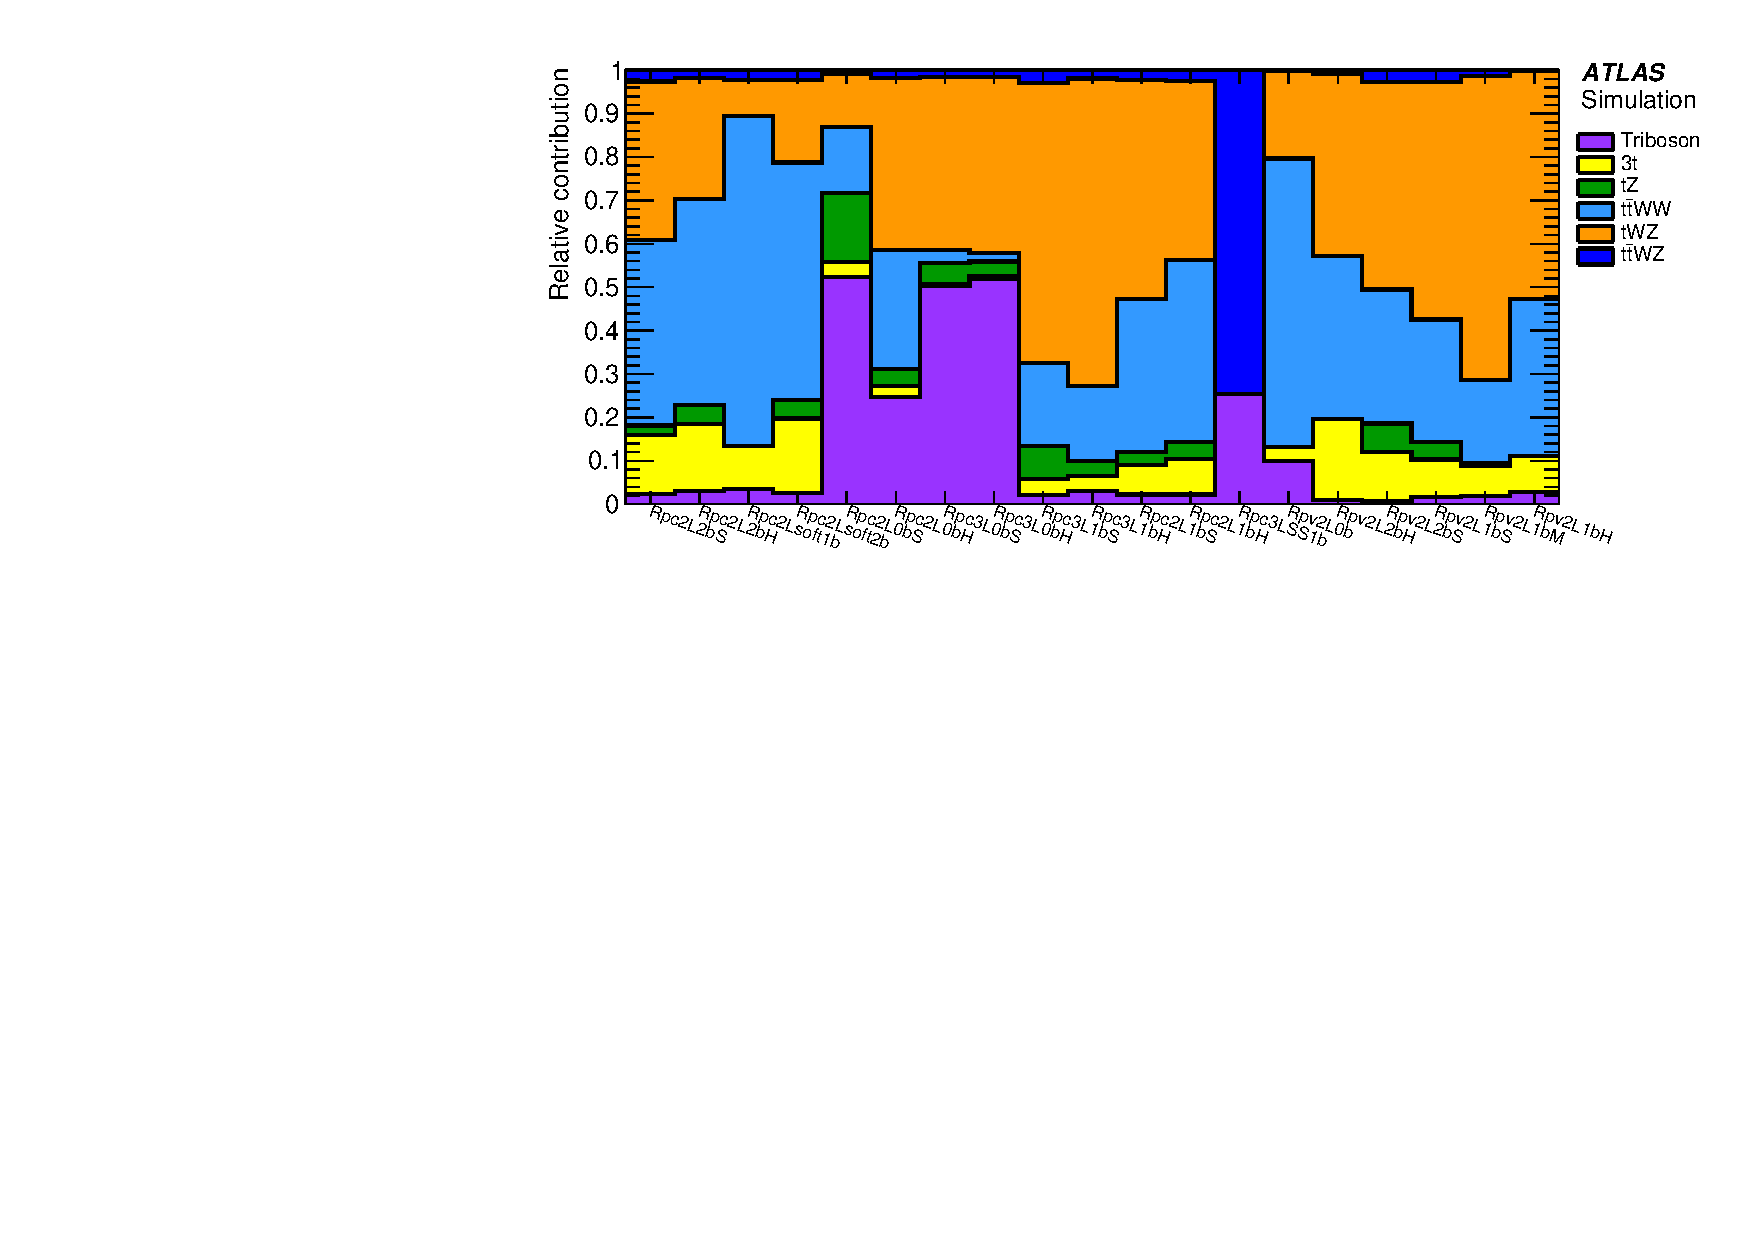
\includegraphics[width=0.9\textwidth]{rareFancy}
\caption{Relative contribution in each signal region from the processes in the category labelled as rare in the paper ($\ttbar WW$, 
$\ttbar WZ$, $tZ$, $tWZ$, $t\ttbar$, $WH$, $ZH$ and triboson production). }
\label{fig:RareBreakdown} 
\end{figure} 

\subsection{Validation regions}
\label{sec:bkg.irred.def}

Dedicated validation regions are defined to verify the estimate
of the $W^\pm W^\pm jj$, the $WZjjjj(j)$, the $\ttbar W$ and $\ttbar Z$ 
processes in the signal regions. 
For a better validation of $WZ$ processes in association with a large jet 
multiplicity, two VRs are proposed : $WZ$4j and $WZ$5j, with 4 and
respectively 5 reconstructed jets in the event.
The corresponding selections are summarized in Table~\ref{tab:VRdef}.

\par{\bf $W^\pm W^\pm$+jets validation region\\}
The $W^{\pm}W^{\pm}$ + jets processes contribute mainly in the signal regions with no $b$-tagged jet requirement and two same-sign leptons. This validation region, $W^\pm W^{\pm}$-VR, has exactly one SS pair (and no additional baseline leptons), zero $b$-jets and at least two jets with \pt above 50 \GeV. Additional requirements on \met\ and \meff\ help to decrease the amount of detector background as shown in Figure~\ref{fig:WW_VR_afterLepJetSel} (left and middle). To further improve the purity, the sub-leading lepton \pt is increased to 30 \GeV, and cuts on minimum angular separation between the leptons and jets, and between the two leptons (Figure~\ref{fig:WW_VR_afterLepJetSel}, right) are placed as detailed in Table~\ref{tab:VRdef}. The purity is around 34\% with this definition 
of the validation region. Signal contamination (highly reduced by applying a veto of all SRs) it is found to be at most 5\% when looking at $\gluino \rightarrow q\bar q (\tilde \ell \ell / \tilde \nu \nu)$ scenarios.

\begin{figure}[t!]
\centering
\begin{subfigure}[t]{0.32\textwidth}
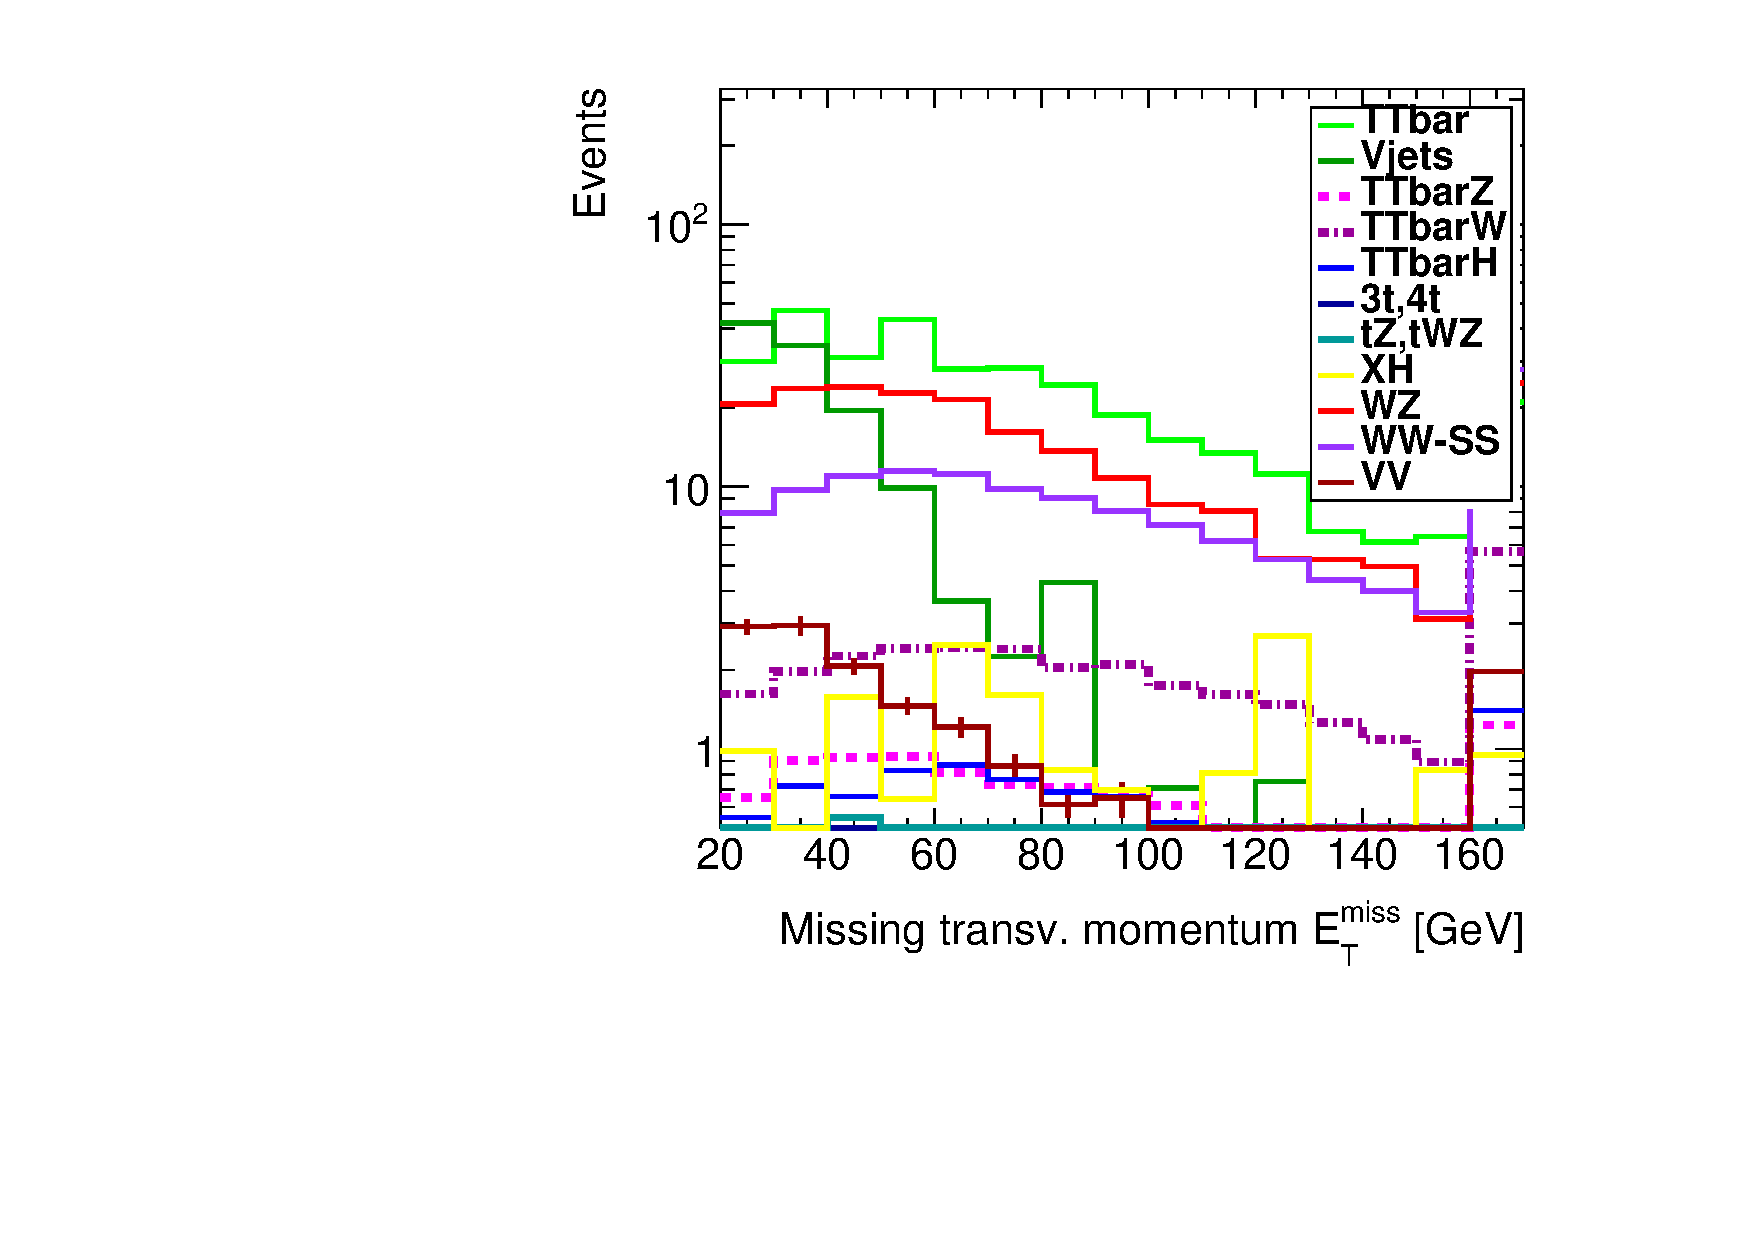
\includegraphics[width=\textwidth]{met_SR42}
\end{subfigure}
\begin{subfigure}[t]{0.32\textwidth}
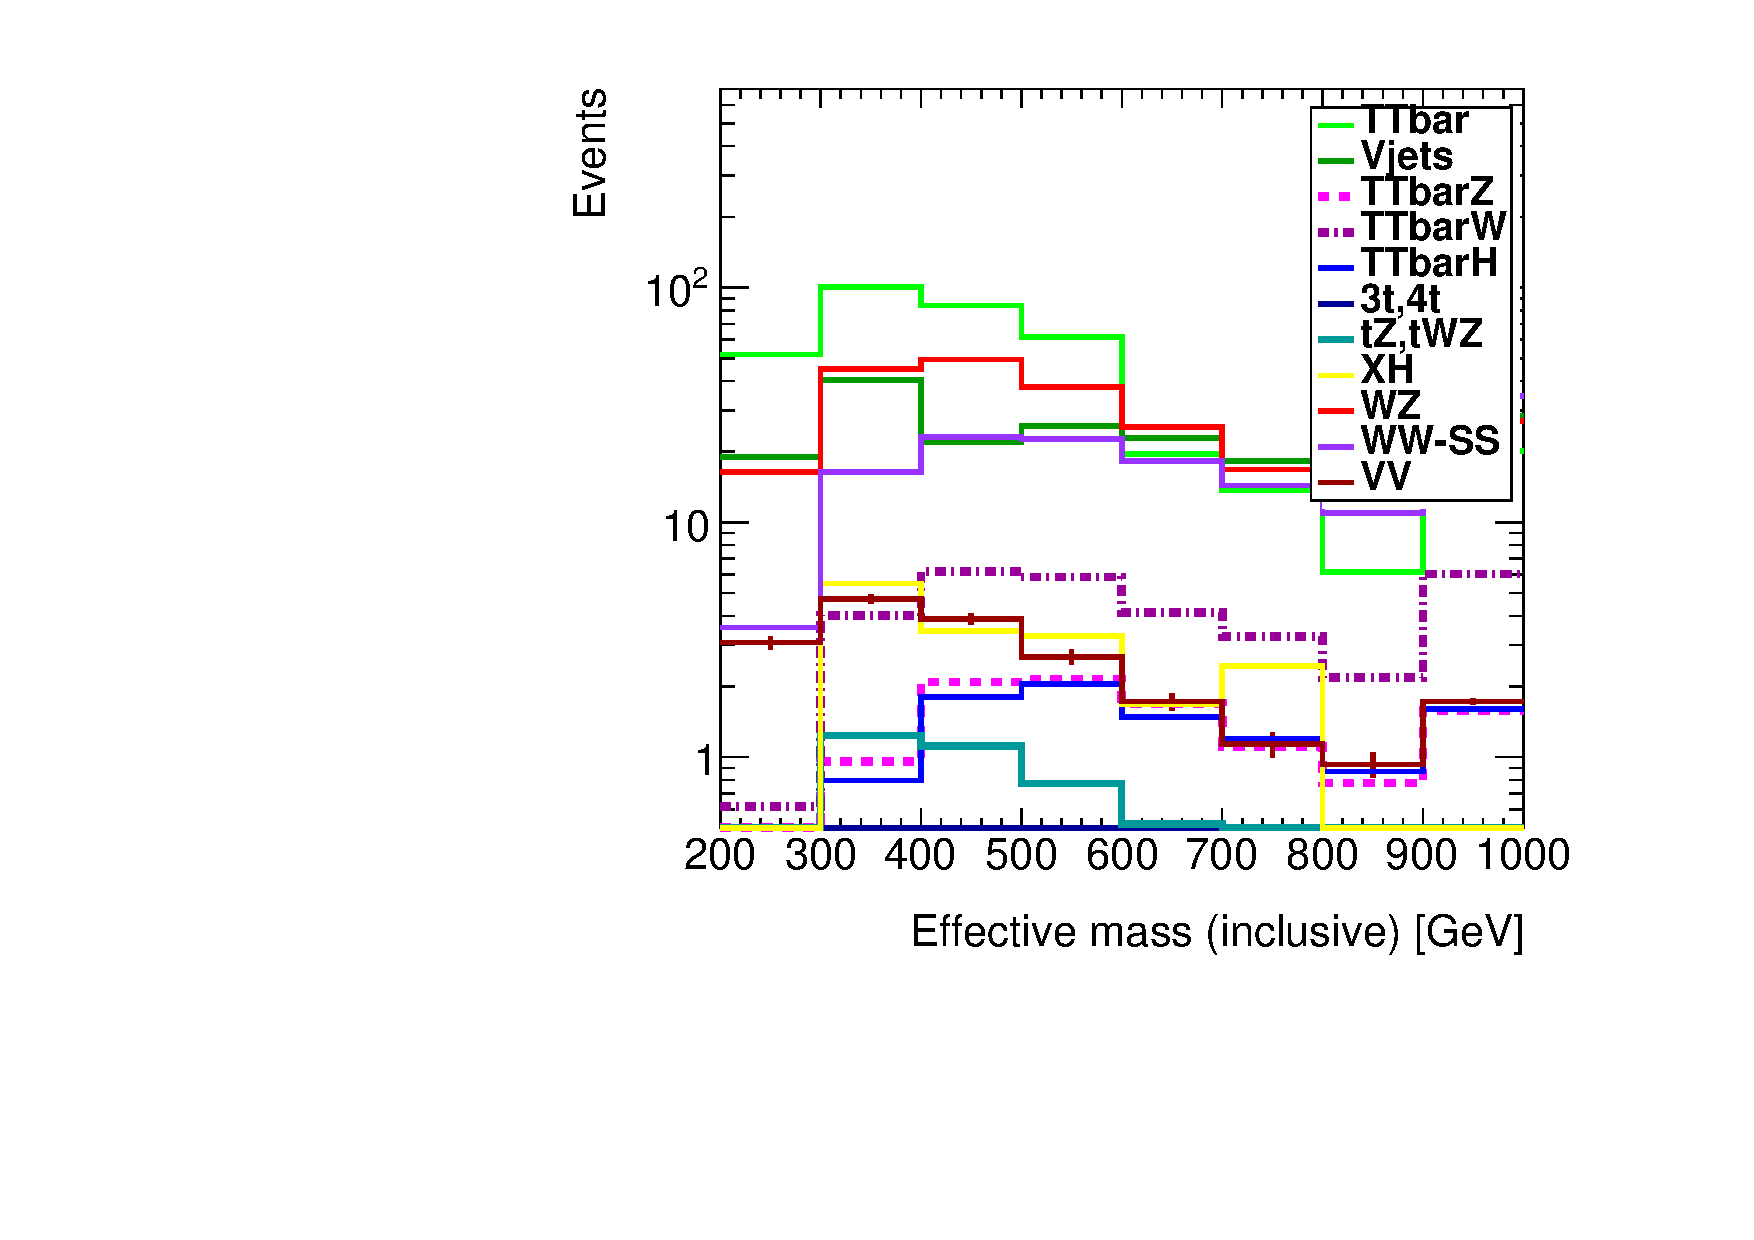
\includegraphics[width=\textwidth]{meff_SR42}
\end{subfigure}
\begin{subfigure}[t]{0.32\textwidth}
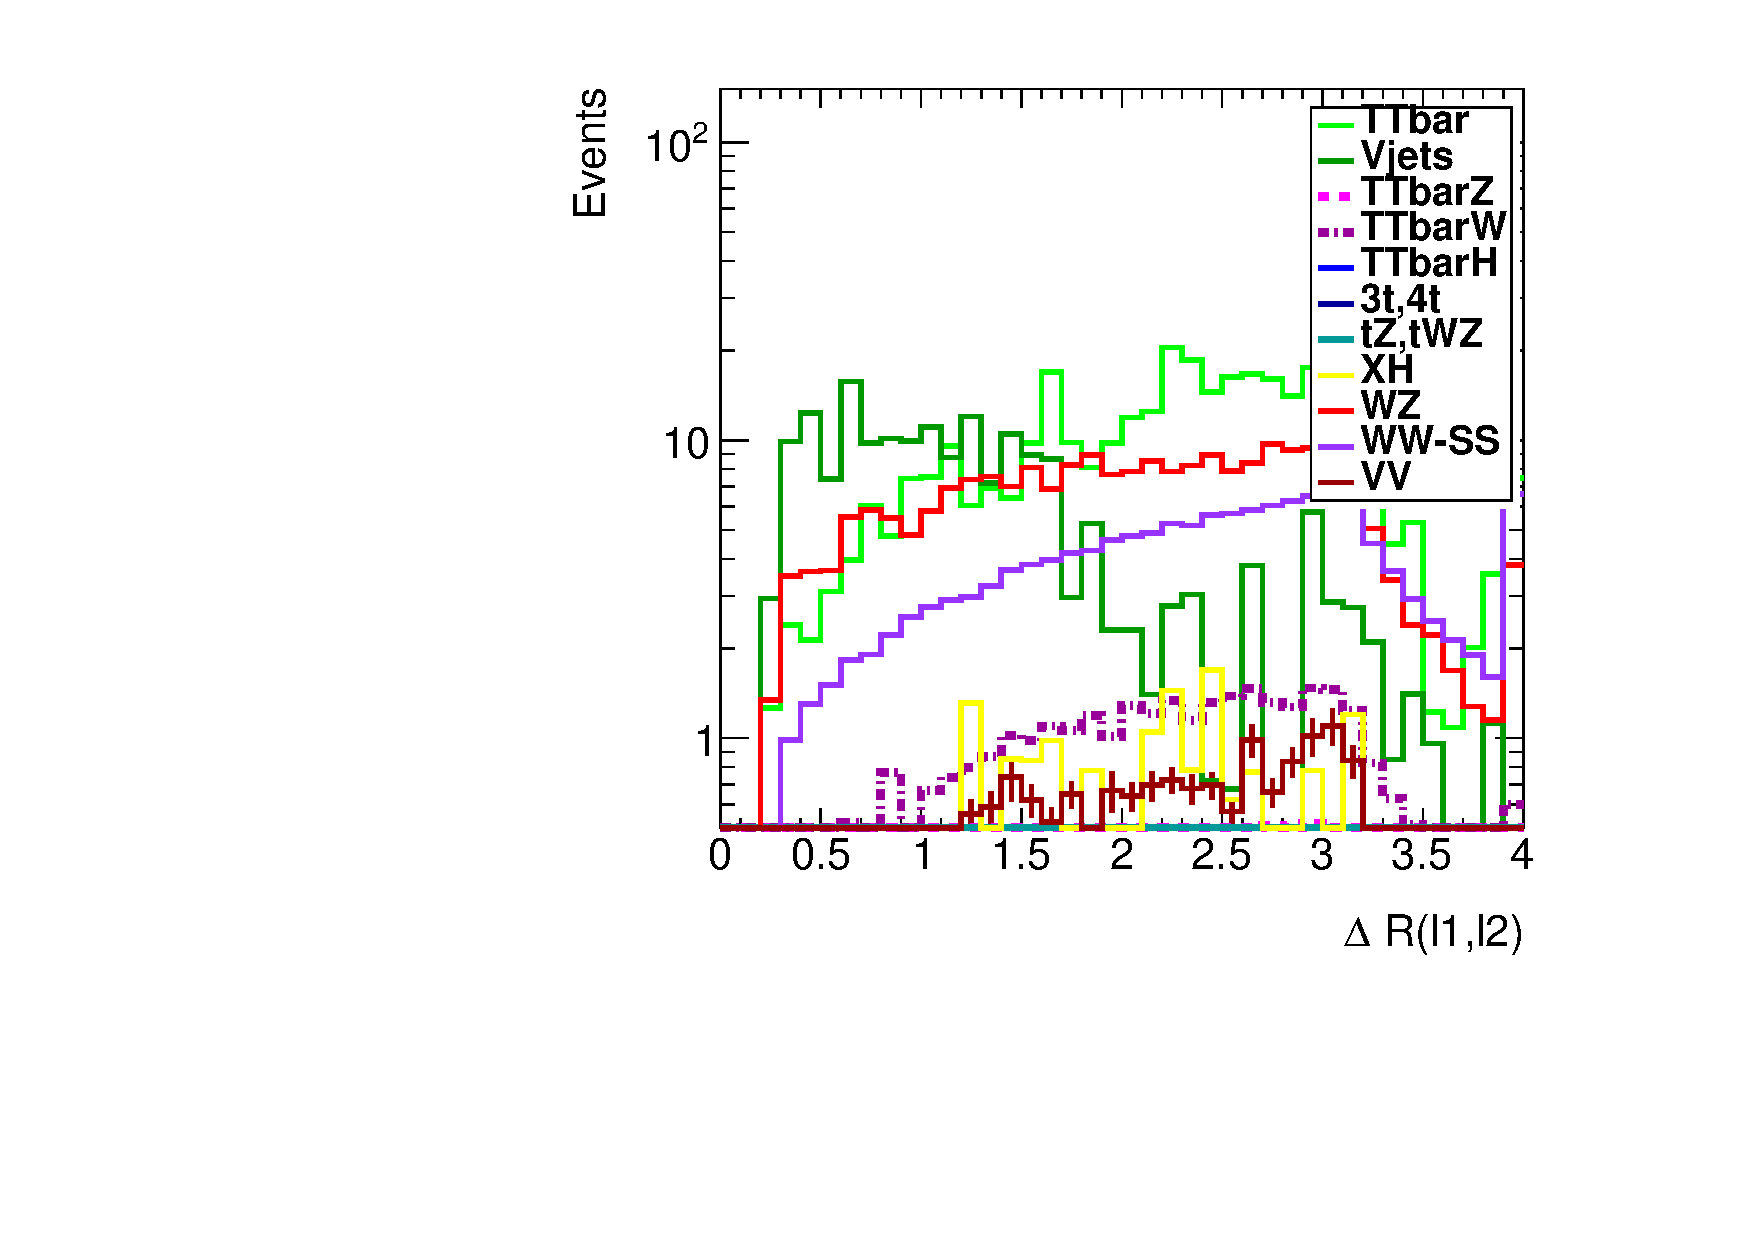
\includegraphics[width=\textwidth]{deltaR_lep1lep2_SR42}
\end{subfigure}
\caption{\met\ (left), \meff\ (middle) and $\operatorname{min}\Delta R (\ell_{1}, \ell_2)$ (right) after lepton and jet selection of the $W^\pm W^\pm$-VR (and no additional requirements). Signal regions are vetoed. All MC samples are normalized to a luminosity of 36.1 \ifb. The last bin includes overflow.
}
\label{fig:WW_VR_afterLepJetSel}
\end{figure} 


%%%%%
\par{\bf $WZ$ + jets validation region\\}
Contributions from $WZ$+jets processes can be significant in regions vetoing the presence of $b$-jets and requiring three leptons. 
Given the large data sample collected, it is possible to design validation 
regions that require at least four and even at least five jets with \pt~$>$25 \GeV~in the event. Thus, two validation regions, $WZ$4j-VR and $WZ$5j-VR, are proposed to better probe the modelling of the jet multiplicity in $WZ$ processes. Both regions are defined with exactly three signal leptons and no fourth baseline lepton, to reduce the $ZZ$ background contamination. The \meff, and the upper cut on the ratio between the \met\ in the event and the sum of all lepton \pt are great discriminants against the reducible backgrounds. Some kinematic distributions after lepton and four jet selection are shown in Figure~\ref{fig:WZ_VR_afterLepJetSel}.

\begin{figure}[t!]
\centering
\begin{subfigure}[t]{0.32\textwidth}
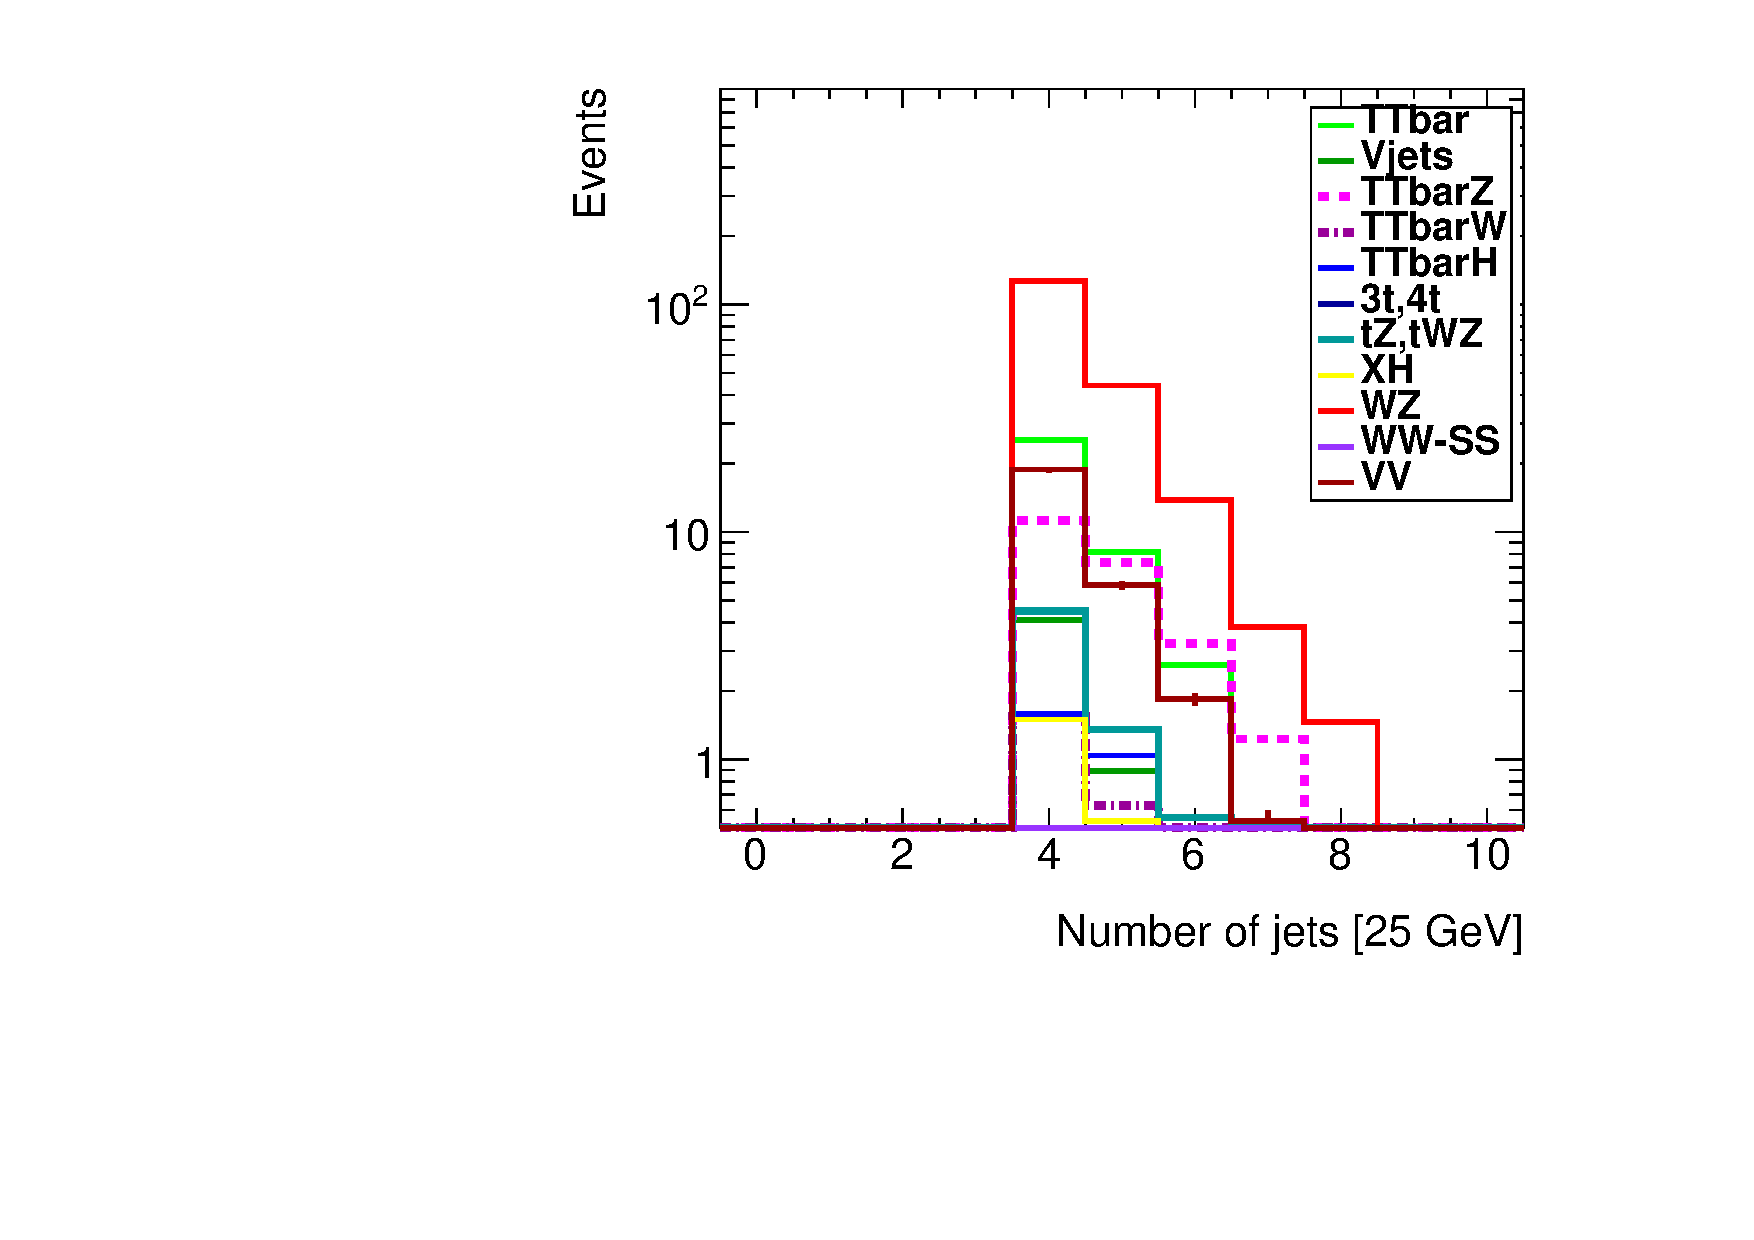
\includegraphics[width=\textwidth]{nJets25_SR32}
\end{subfigure}
\begin{subfigure}[t]{0.32\textwidth}
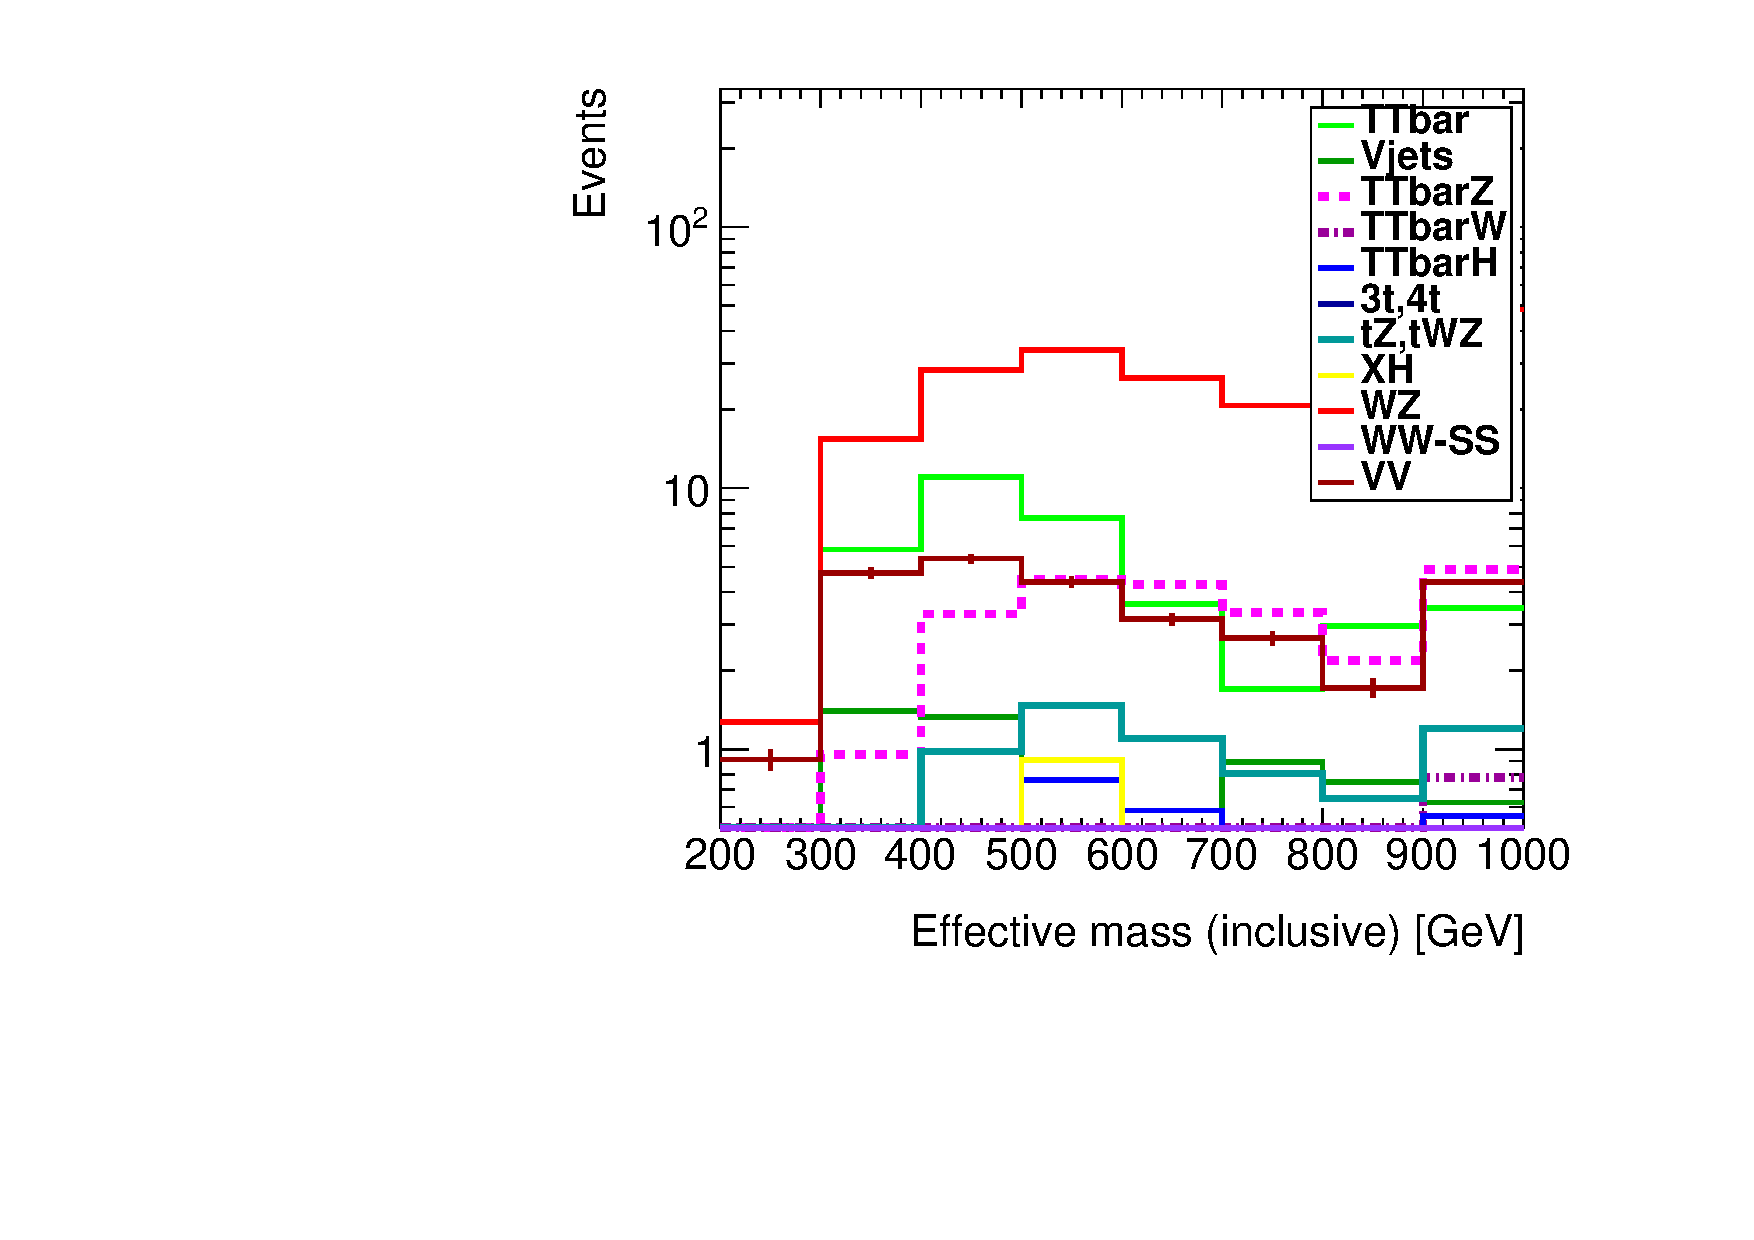
\includegraphics[width=\textwidth]{meff_SR32}
\end{subfigure}
\begin{subfigure}[t]{0.32\textwidth}
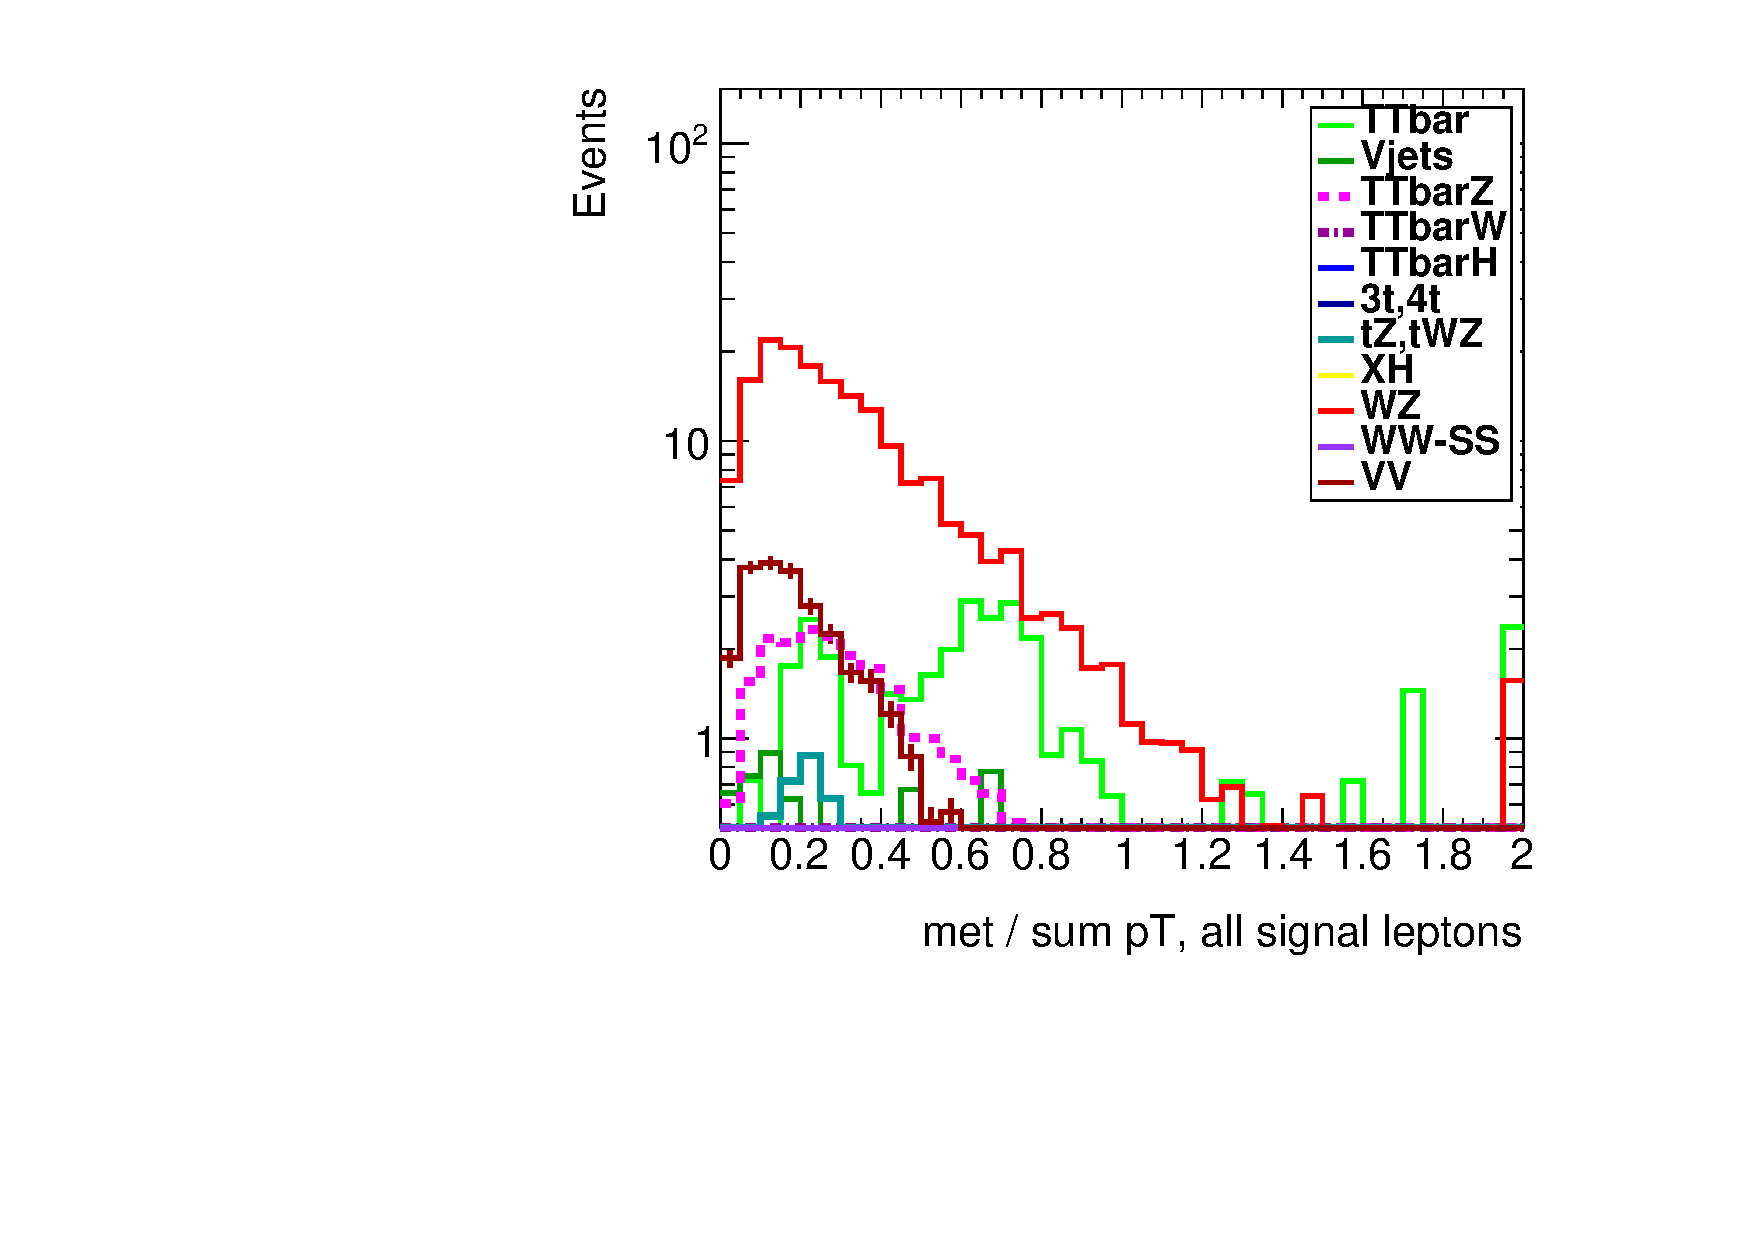
\includegraphics[width=\textwidth]{metOverpTallLep_signal_SR32}
\end{subfigure}
\caption{Number of jets with \pt $>$ 25 \GeV~(left), \meff\ (middle) and ratio between the \met\ in the event and the sum of all lepton \pt (right) after lepton and four jet selection of the $WZ$-VR (and no additional requirements). Signal regions are vetoed as detailed in Table~\ref{tab:VRdef}. All MC samples are normalized to a luminosity of 36.1 \ifb. The last bin includes overflow.
}
\label{fig:WZ_VR_afterLepJetSel}
\end{figure} 

Purity in $WZ$4j-VR ($WZ$5j-VR) is around 67$\%$ (64\%). When looking at $\gluino \rightarrow q \bar q (\tilde \ell \ell / \tilde \nu \nu)$ scenarios, the signal contamination is below 5\% in most of the non-excluded phase space, except for small $\Delta M(\gluino,\neut)$ where it can go up to 30\% (15\%). Signal contamination is found to be much lower for $\gluino \rightarrow q \bar q WZ \neut$ scenarios.



%%%%%
\par{\bf \ttbar\ + $W$ background validation\\}
A \ttbar\ + $W$ validation region ($\ttbar W$-VR) is defined with exactly one SS lepton pair and at least one $b$-jet. At least four jets are required in the $ee$ and $e\mu$ channels, while in the $\mu\mu$ channel the selection is relaxed to at least three jets  (less reducible background); also the jet \pt thresholds are different between these two cases (same motivation). As shown in Figure~\ref{fig:ttW_VR_afterLepJetSel}, the amount of \ttbar\ background after this pre-selection is still very large and additional requirements on \met, \meff\ and on the ratio between the sum of \pt of all $b$-jets and the sum of \pt of all jets are placed as mentioned in Table~\ref{tab:VRdef}. With this definition the achieved purity in $\ttbar W$-VR is 33\%. 
Signal contamination is around 20\% when looking at $\tilde b\tilde b$ SUSY 
models.

\begin{figure}[t!]
\centering
\begin{subfigure}[t]{0.32\textwidth}
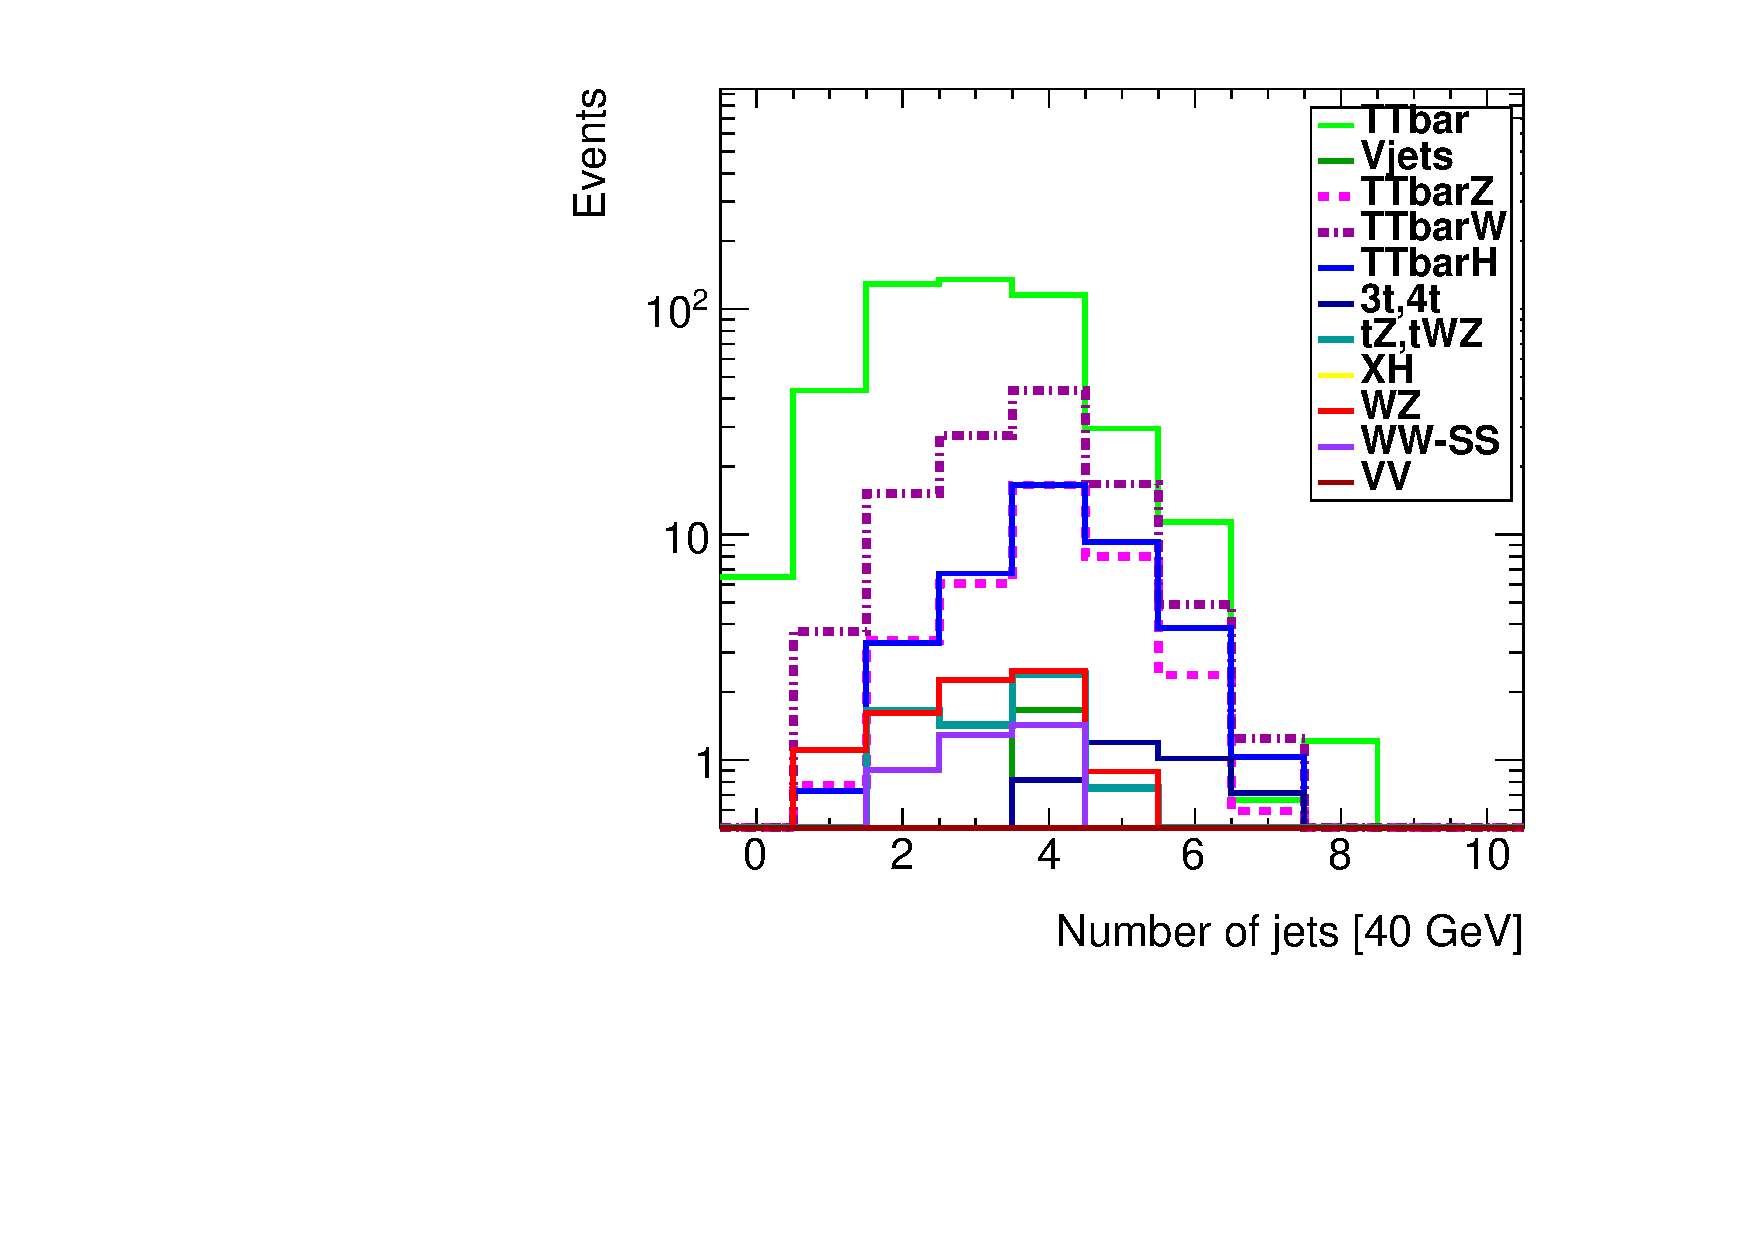
\includegraphics[width=\textwidth]{nJets40_SR2}
\end{subfigure}
\begin{subfigure}[t]{0.32\textwidth}
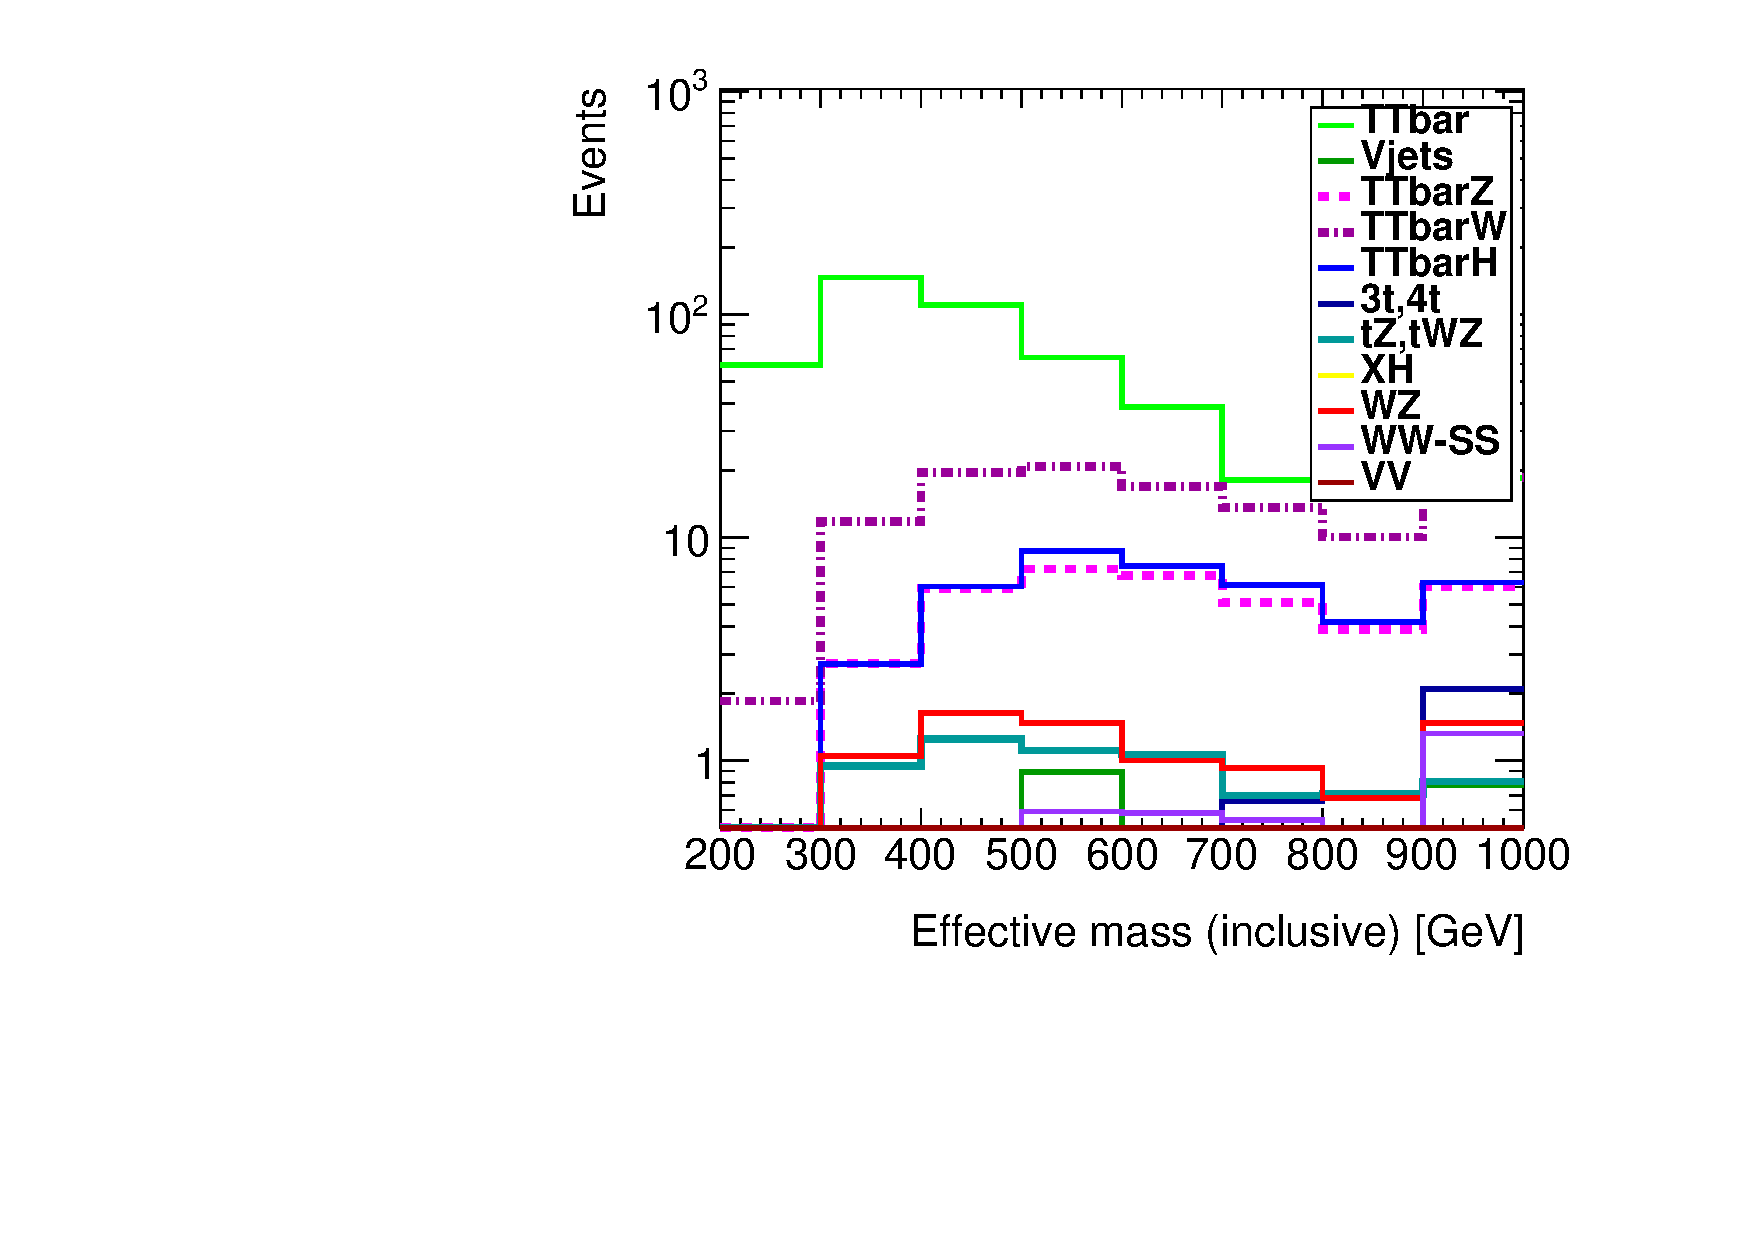
\includegraphics[width=\textwidth]{meff_SR2}
\end{subfigure}
\begin{subfigure}[t]{0.32\textwidth}
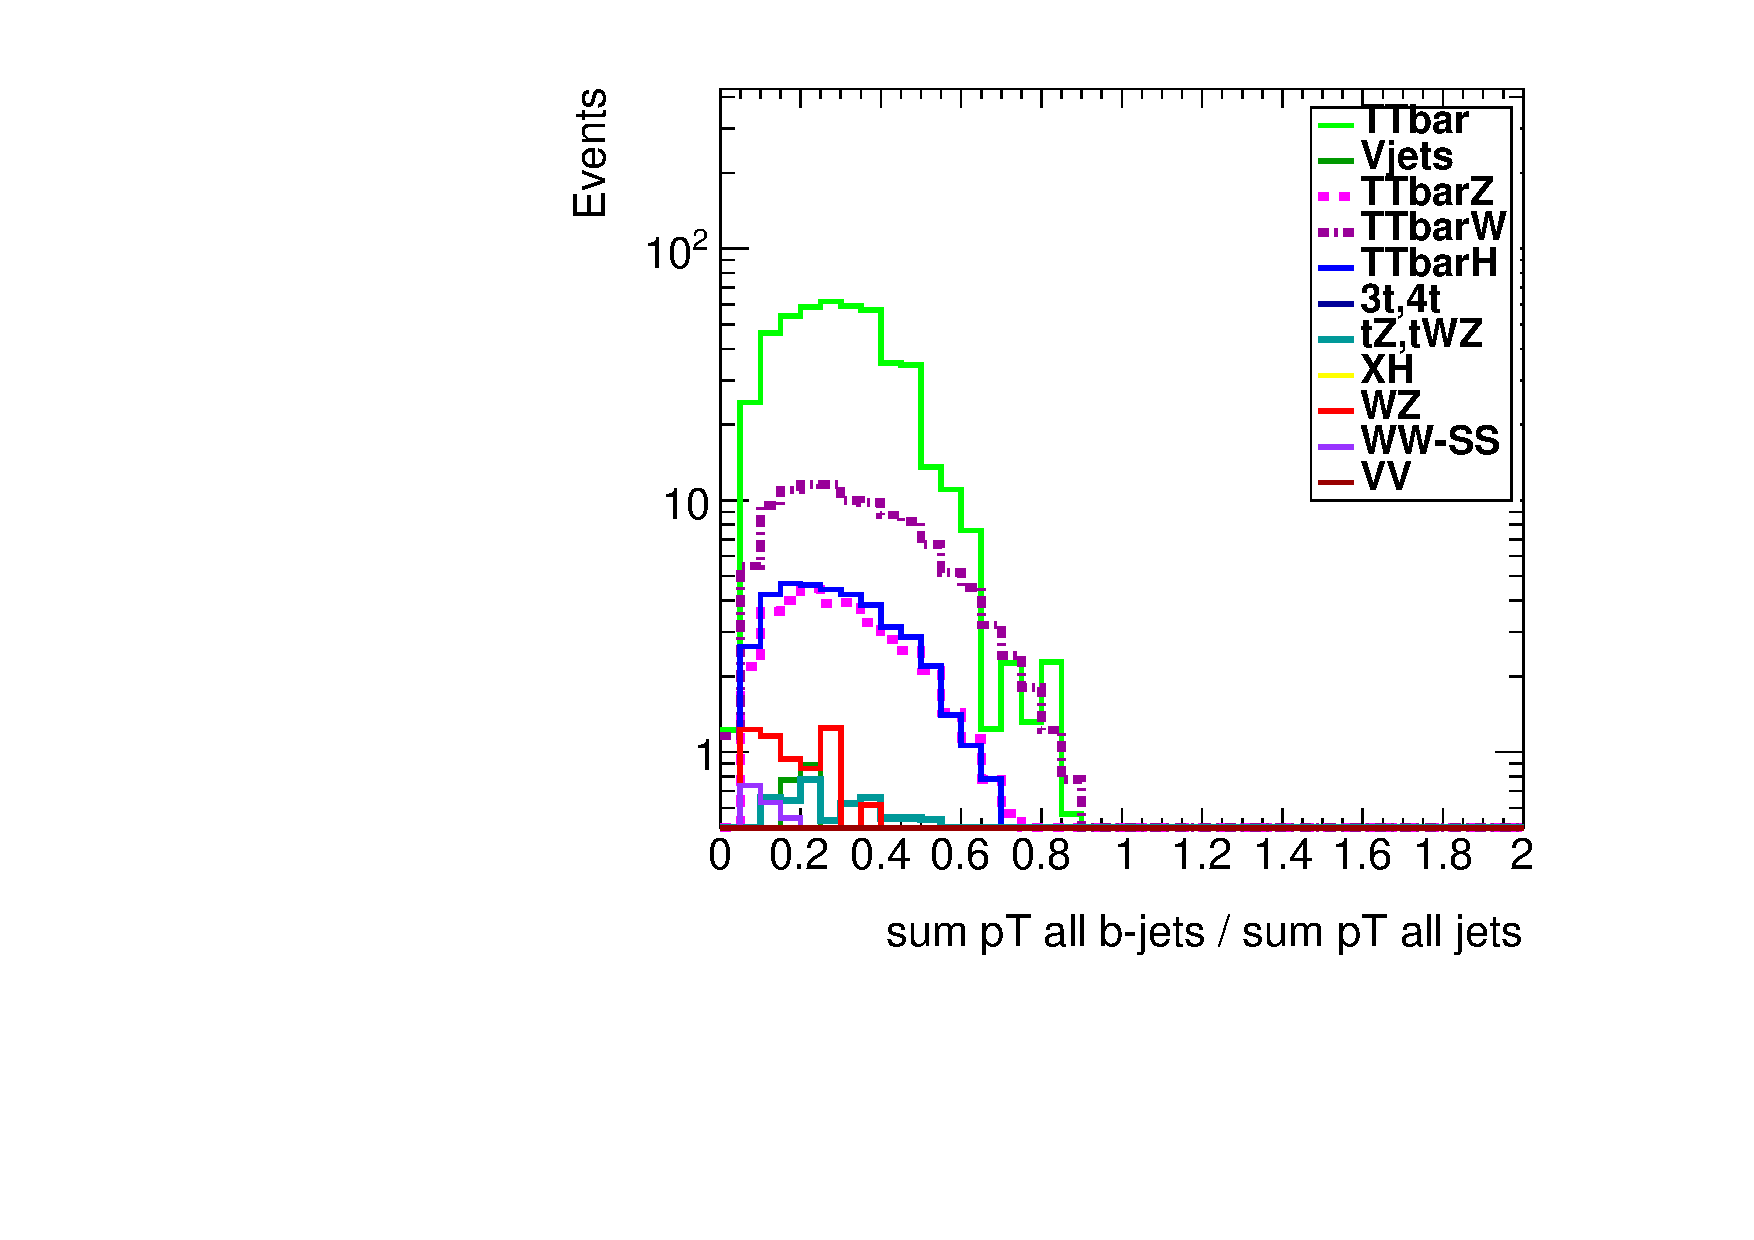
\includegraphics[width=\textwidth]{pTallBJets_over_pTallJets_SR2}
\end{subfigure}
\caption{Number of jets with \pt $>$ 40 \GeV~(left), \meff\ (middle) and ratio between the sum of all $b$-jets \pt and the sum of all jets \pt (right) after lepton and jet selection of the $\ttbar W$-VR (and no additional requirements). Signal regions are vetoed as detailed in Table~\ref{tab:VRdef}. All MC samples are normalized to a luminosity of 36.1 \ifb. The last bin includes overflow.
}
\label{fig:ttW_VR_afterLepJetSel}
\end{figure} 

%%%%%
\par{\bf \ttbar\ + $Z$ background validation\\}
A \ttbar\ + $Z$ enriched validation region ($ttZ$-VR) is defined with at least one SFOS lepton pair and at least one $b$-jet. At least three jets are required in the event regardless of the lepton channel. Some kinematic distributions after this pre-selection are shown in Figure~\ref{fig:ttZ_VR_afterLepJetSel} (left and middle). To increase the purity, the invariant mass of the SFOS lepton pair is selected to be inside the $[81, 101]$ \GeV~interval and the \meff\ in the event should be greater than 450 \GeV. With this selection, the purity is 58\%. One can increase it even further (by $\sim$10\%) if at least two $b$-jets are required in the event. However, with such a cut the statistics will be highly reduced (up to a factor 2 lower as illustrated in Figure~\ref{fig:ttZ_VR_afterLepJetSel}, right), so it is not pursued. The signal contamination is found to be around 5\% for \sbsb\ pair production.

\begin{figure}[t!]
\centering
\begin{subfigure}[t]{0.32\textwidth}
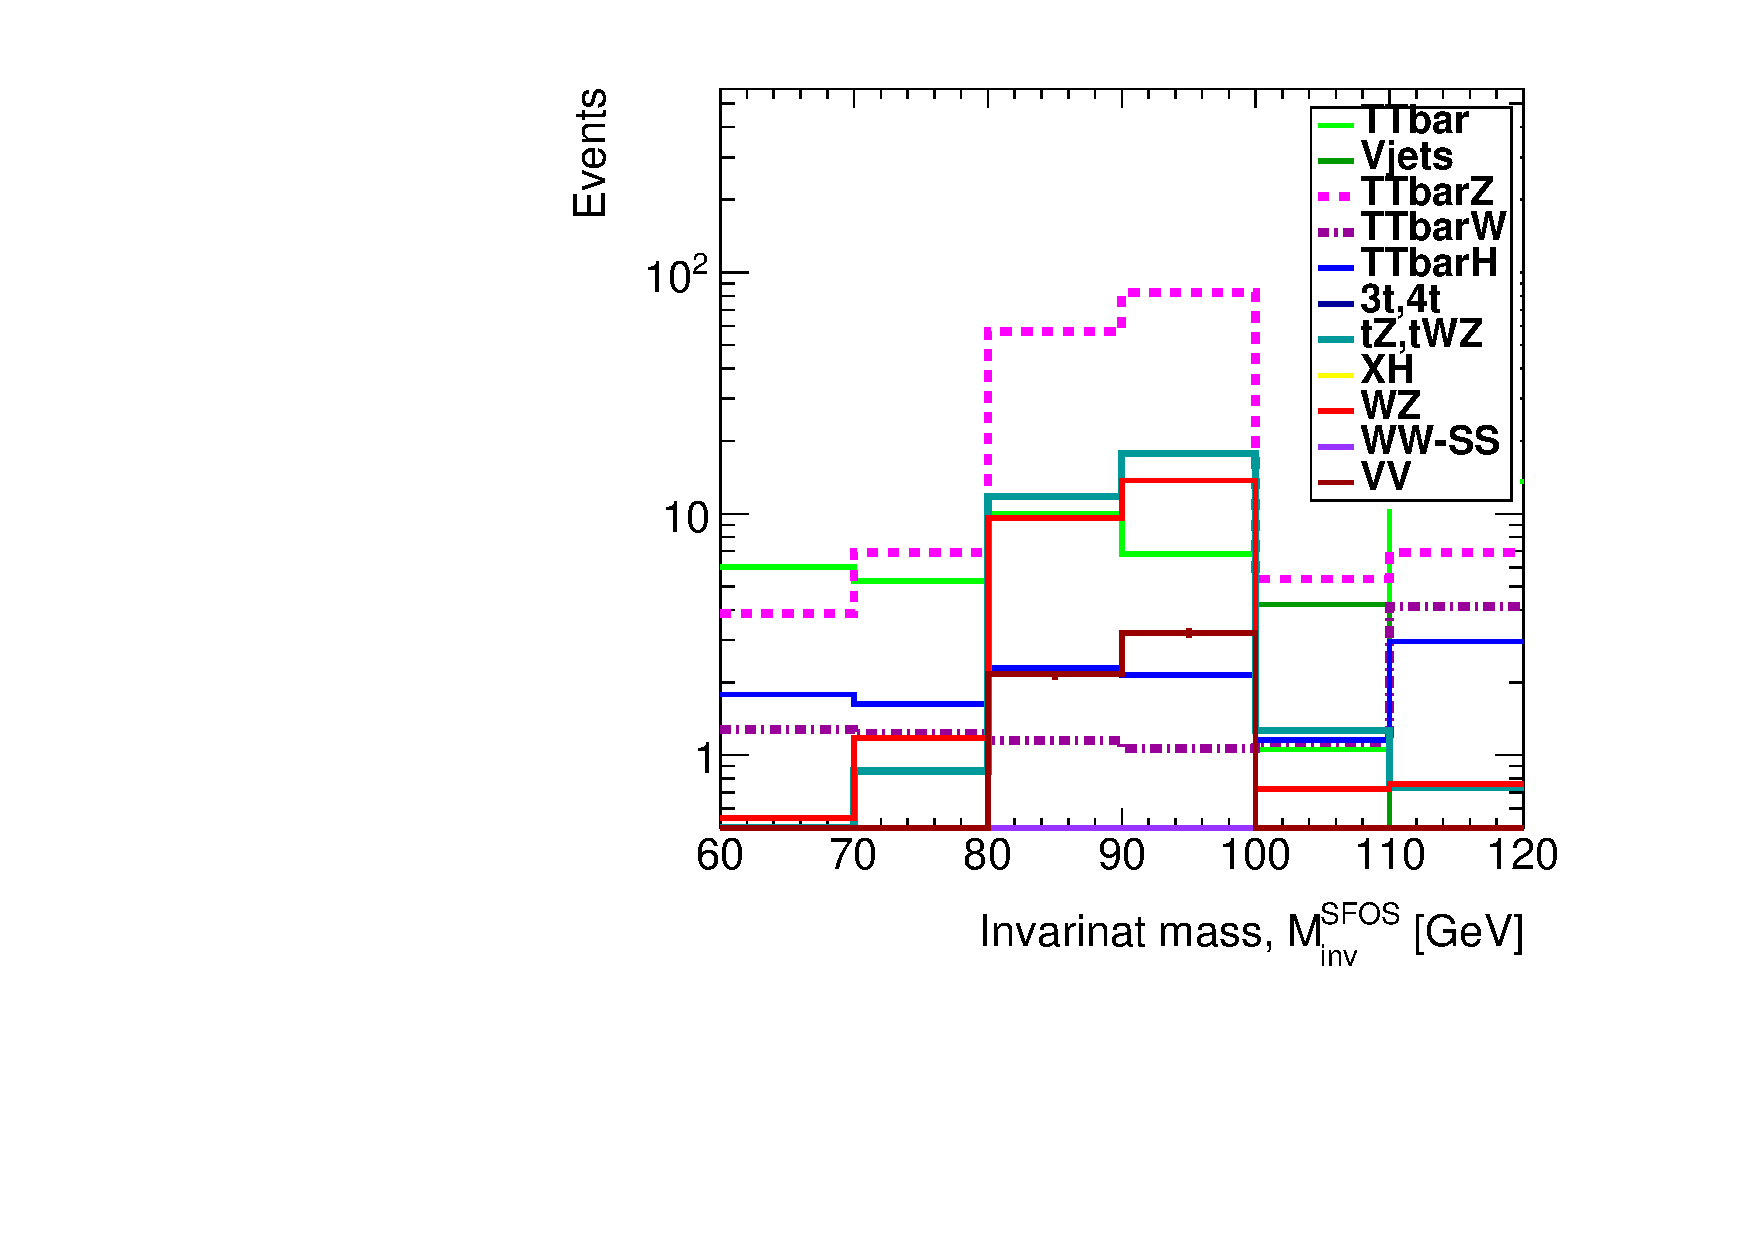
\includegraphics[width=\textwidth]{mSFOS_SR12}
\end{subfigure}
\begin{subfigure}[t]{0.32\textwidth}
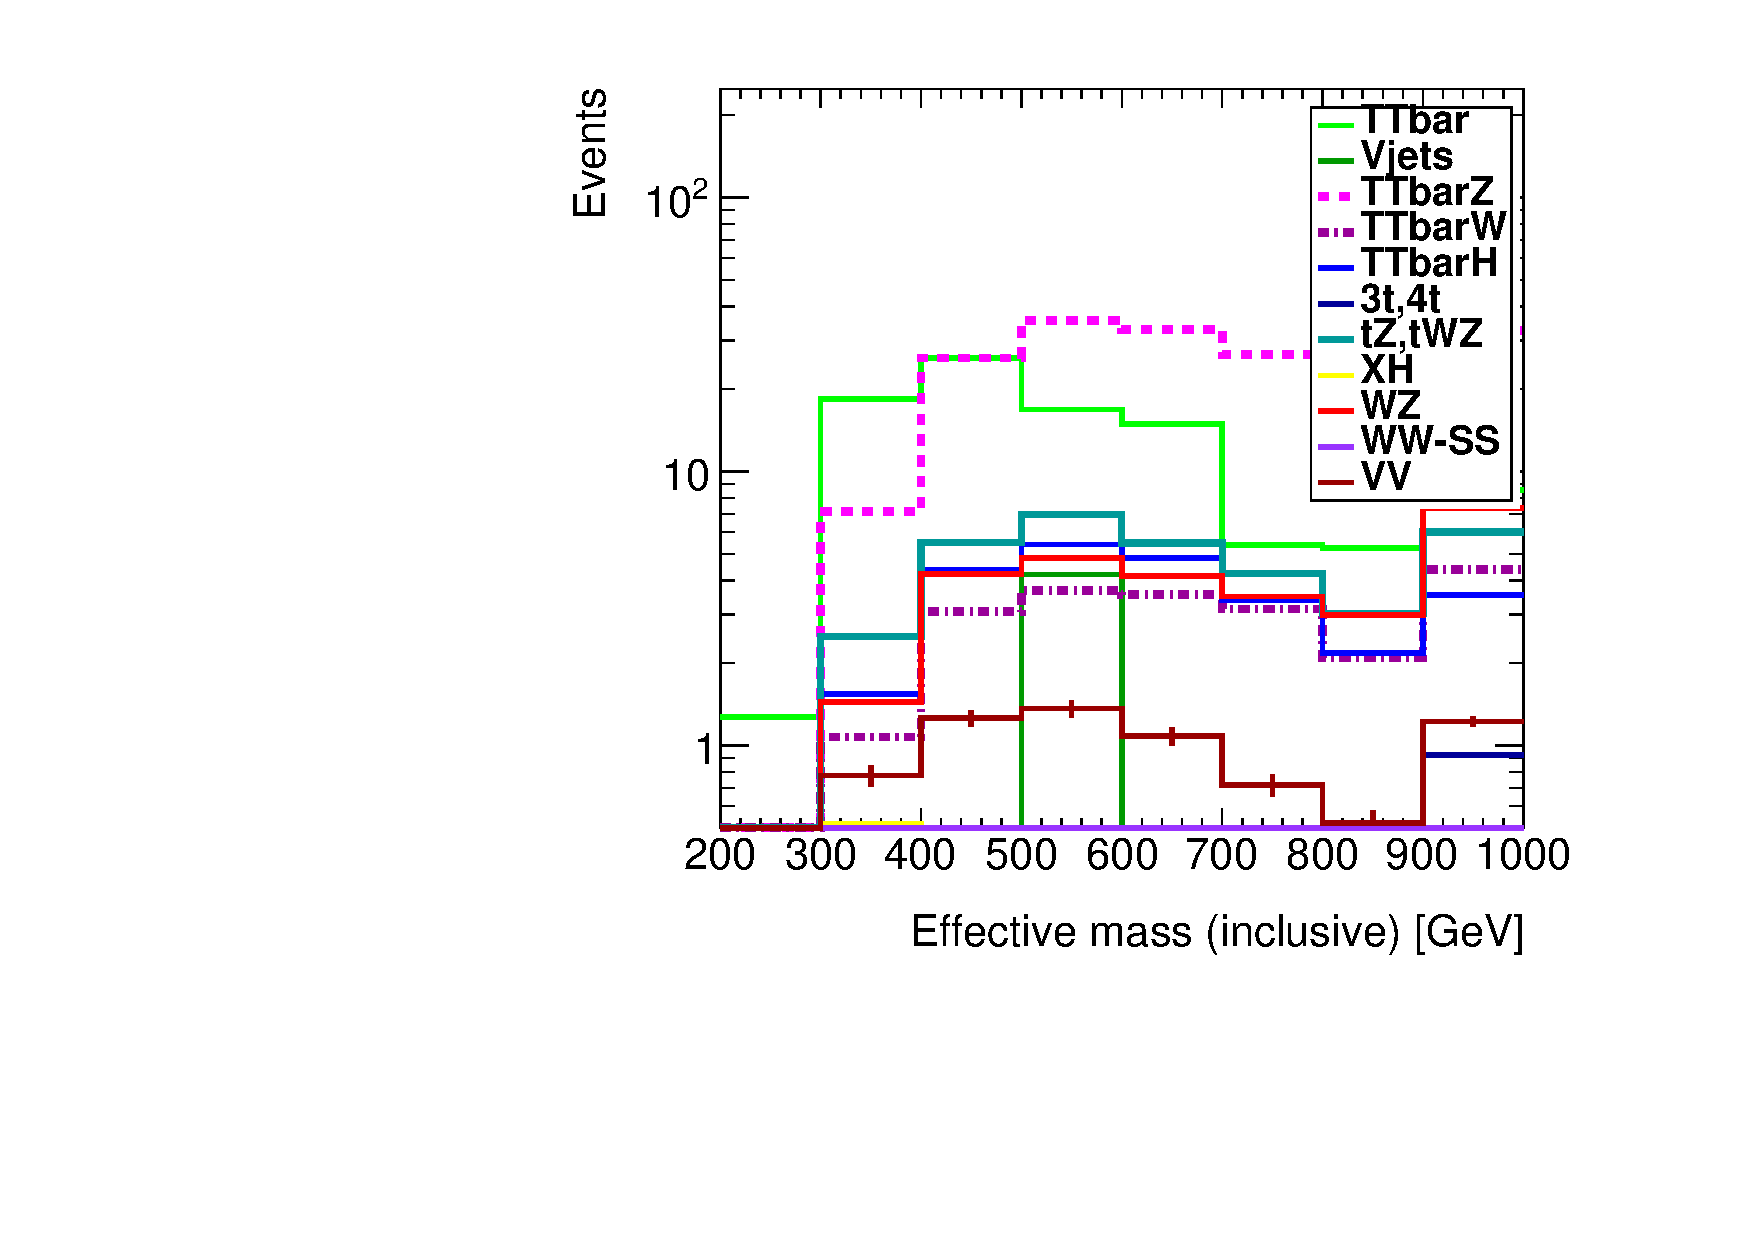
\includegraphics[width=\textwidth]{meff_SR12}
\end{subfigure}
\begin{subfigure}[t]{0.32\textwidth}
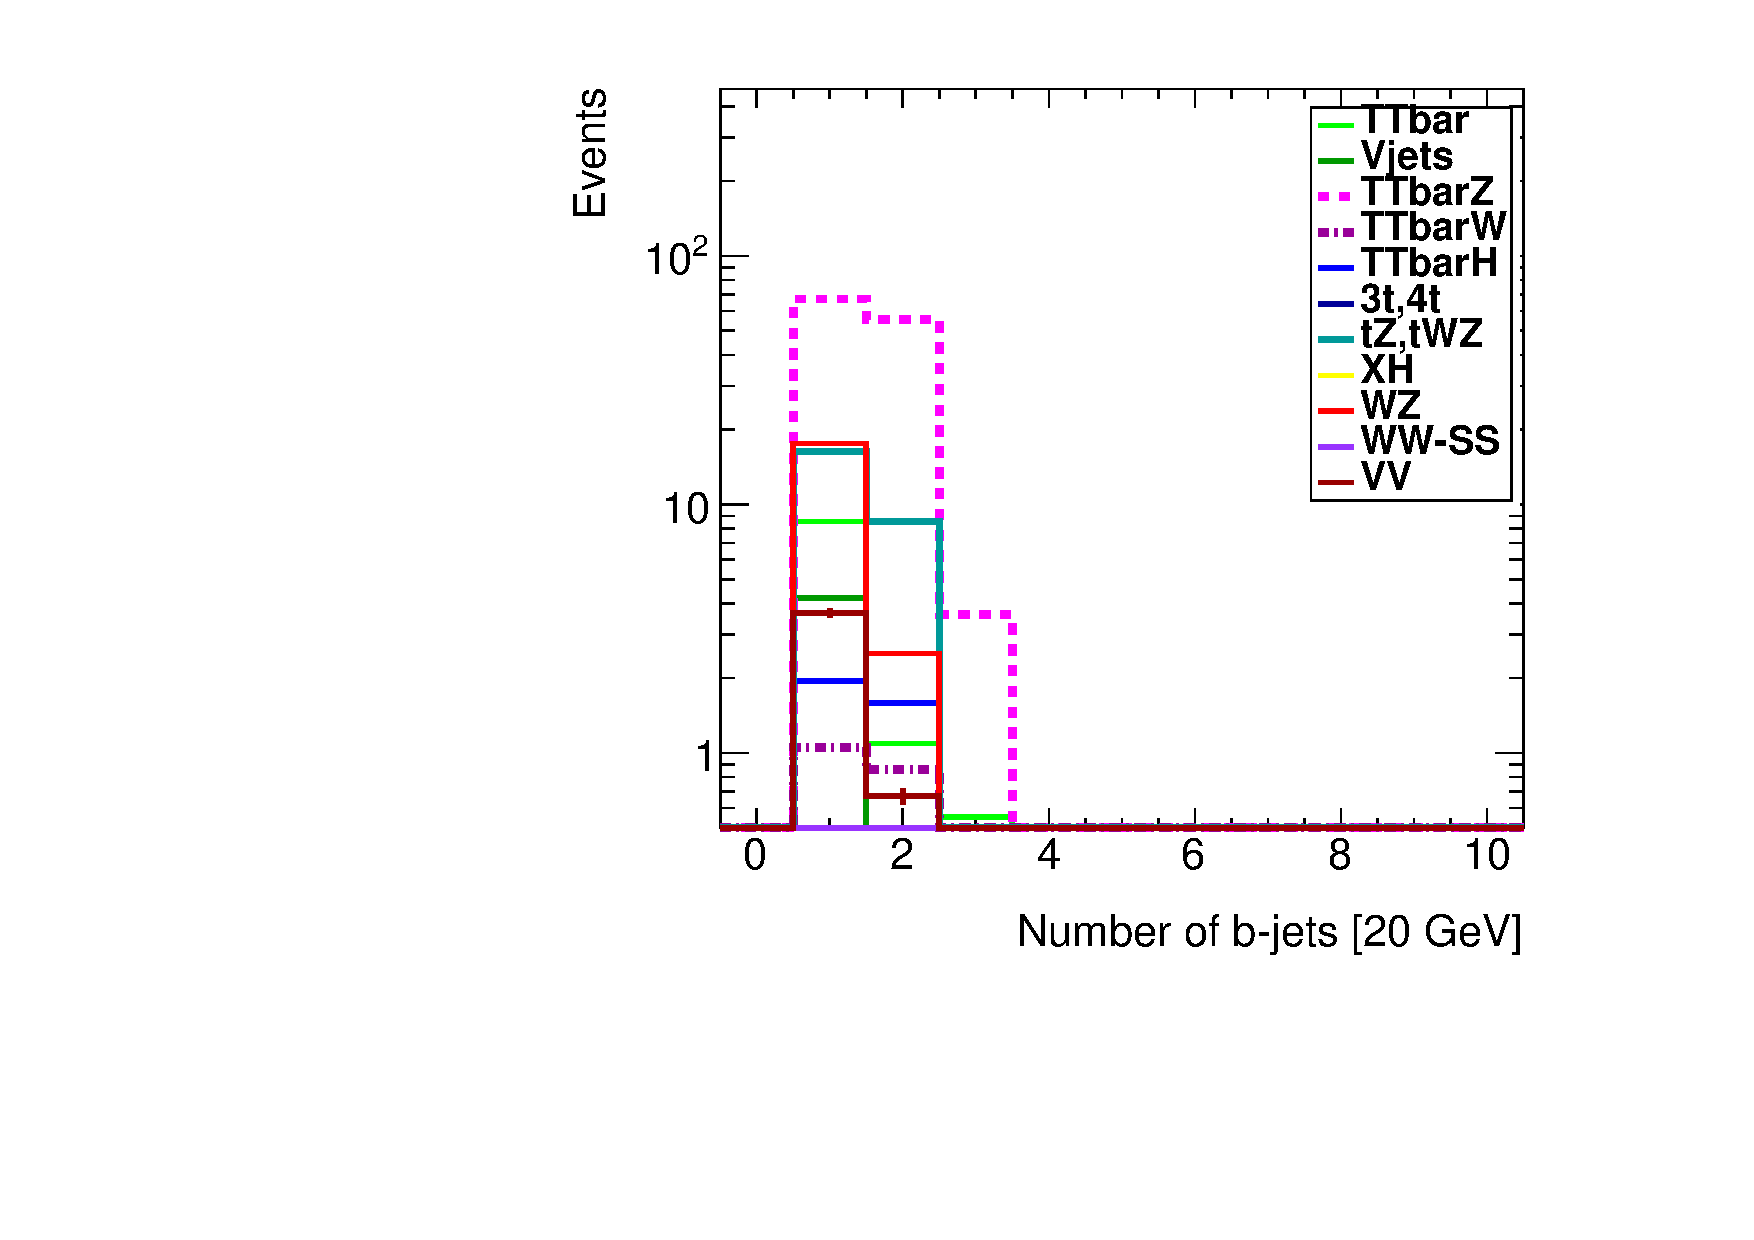
\includegraphics[width=\textwidth]{nBJets20_SR13}
\end{subfigure}
\caption{Invariant mass of the SFOS lepton pair (left) and \meff\ (middle) after lepton and jet selection of the $\ttbar Z$-VR (and no additional requirements). Number of $b$-jets with \pt $>$ 20 \GeV~after the $\ttbar Z$-VR selection. Signal regions are vetoed as detailed in Table~\ref{tab:VRdef}. All MC samples are normalized to a luminosity of 36.1 \ifb. The last bin includes overflow.
}
\label{fig:ttZ_VR_afterLepJetSel}
\end{figure} 


\begin{table}[t!]
\hspace{0.5cm}
\def\arraystretch{1.1}
\centering
\resizebox{\textwidth}{!}
{\small
\begin{tabular}{|l|c|c|c|c|c|c|c|}
\hline    
Validation        &  $N_{\textrm{leptons}}^{\textrm{signal}}$    & $N_{b\textrm{-jets}}$  &  $N_{\textrm{jets}}$  & $\pt^{\textrm{jet}}$  & \met\ & \meff\  & Other \\
Region            &  &  &  & [GeV]  & [GeV] & [GeV]  & \\
\hline\hline
$\ttbar W$   	&$=2SS$     &$\geq 1$   & $\geq 4$ ($e^\pm e^\pm$, $e^\pm \mu^\pm$) & $>40$ & $> 45$  & $> 550$   & $\pt^{\ell_2}>40$~GeV\\
              	&           &       &  $\geq 3$ ($\mu^\pm \mu^\pm$)   &  $>25$ &      &          & $\sum \pt^{b\textrm{-jet}}/\sum \pt^{\textrm{jet}}>0.25$ \\ 
\hline
$\ttbar Z$    	&$\geq 3$  & $\geq 1$ & $\geq 3$ &  $>35$ &  --    & $> 450$  & $81<m_\text{SFOS}<101$~GeV~\\
                &$\geq 1$ SFOS pair&     &          &       &         &         &  \\
\hline
$WZ$4j            & $=3$      &  $=0$ & $\geq 4$ &  $>25$   & --    & $> 450$ & $\met/\sum \pt^{\ell} < 0.7$ \\
\hline
$WZ$5j            & $=3$      &  $=0$ & $\geq 5$ &  $>25$   & --    & $> 450$ & $\met/\sum \pt^{\ell} < 0.7$  \\ 
\hline
$W^{\pm} W^{\pm}jj$ & $=2SS$      &  $=0$ & $\geq 2$ &   $>50$ & $> 55$  & $> 650$ & veto $81<\mee<101$~GeV~ \\
               	  &               &	  &	     &         &   	&	  & $\pt^{\ell_2}>30$~GeV~\\
               	  &		  &	  &	     &         &   	&	  & $\Delta R_\eta (\ell_{1,2},j)>0.7$  \\
               	  &		  &	  &	     &         &   	&	  & $\Delta R_\eta (\ell_1, \ell_2)>1.3$ \\
\hline
All VRs           & \multicolumn{7}{c|}{Veto events belonging to any SR} \\
\hline
\end{tabular}
}
\caption{Summary of the event selection in the validation regions (VRs). 
Requirements are placed on the number of signal leptons ($N_{\textrm{leptons}}^{\textrm{signal}}$), 
the number of $b$-jets with $\pt>20 \GeV$ ($N_{b\textrm{-jets}}$) or the number of jets ($N_{\textrm{jets}}$) 
above a certain \pt threshold ($\pt^{\textrm{jet}}$). The two leading-\pt 
leptons are referred to as $\ell_{1,2}$ with decreasing \pt. Additional requirements are set 
on \met, \meff, the invariant mass of the two leading electrons \mee, the presence of SS 
leptons or a pair of same-flavour opposite-sign leptons (SFOS) and its invariant mass $m_\text{SFOS}$. 
A minimum angular separation between the leptons and the jets ($\Delta R_\eta (\ell_{1,2}, j)$) and between the two 
leptons ($\Delta R_\eta (\ell_{1}, \ell_2)$) is imposed in the $W^\pm W^\pm jj$ VR. 
For the two $WZ$ VRs the selection also relies on the ratio of the \met in the event to the sum of \pt of all signal leptons \pt (\met/$\sum{\pt^{\ell}}$). 
The ratio of the scalar sum of the \pt of all $b$-jets to that of all jets in the event 
($\sum \pt^{b{\textrm{-jet}}} / \sum{\pt^{\textrm{jet}}}$) is used in the $\ttbar W$ VR selection.}
\label{tab:VRdef}
\end{table}

\subsection{Validation of irreducible background estimates}
\label{sec:bkg.irred.res}

The observed yields, compared with the background predictions and uncertainties, 
can be seen in Table~\ref{tab:VR_yields}. There is good agreement between data and the estimated background in all
the validation regions. 

\begin{table}[t!]
\hspace{0.5cm}
\def\arraystretch{1.1}
\centering
\resizebox{\textwidth}{!}{
\begin{tabular}{|l|c|c|c|c|c|}
\hline    
 Validation Region       & $\ttbar W$           & $\ttbar Z$           & $WZ$4j              & $WZ$5j                 & $W^\pm W^{\pm}jj$     \\
\hline\hline
$\ttbar Z/\gamma^*$      & $ 6.2 \pm 0.9 $      & $ 123 \pm 17\hpO $   & $ 17.8 \pm 3.5\hpO$ & $ 10.1\pm 2.3\hpO $    & $ 1.06 \pm 0.22 $     \\
$\ttbar W$               & $ 19.0 \pm 2.9\hpO $ & $ 1.71 \pm 0.27 $    & $ 1.30 \pm 0.32$    & $ 0.45 \pm 0.14 $      & $ 4.1 \pm 0.8 $     \\
$\ttbar H$               & $  5.8 \pm 1.2 $     & $ 3.6 \pm 1.8 $      & $ 1.8 \pm 0.6$      & $ 0.96 \pm 0.34 $      & $ 0.69 \pm 0.14 $     \\
4$t$                     & $ 1.02 \pm 0.22 $    & $ 0.27 \pm 0.14 $    & $ 0.04 \pm 0.02$    & $ 0.03 \pm 0.02 $      & $ 0.03 \pm 0.02 $     \\
$W^{\pm}W^{\pm}$         & $ 0.5 \pm 0.4 $      &   --                 &   --                &   --                   & $ 26 \pm 14$     \\
$WZ$                     & $ 1.4 \pm 0.8 $      & $ 29 \pm 17 $        & $ 200 \pm 110$      & $ 70 \pm 40 $          & $ 27 \pm 14 $    \\
$ZZ$                     & $ 0.04 \pm 0.03 $    & $  5.5 \pm  3.1$     & $ 22 \pm 12$        & $  9\pm 5 $            & $ 0.53\pm 0.30 $     \\
Rare                     & $ 2.2 \pm 0.5 $      & $ 26 \pm 13 $        & $ 7.3 \pm 2.1$      & $  3.0 \pm 1.0 $       & $ 1.8 \pm 0.5 $     \\
Fake/non-prompt leptons  & $ 18 \pm 16$         & $ 22 \pm 14$         & $ 49 \pm 31 $       & $  17 \pm 12 $         & $ 13 \pm 10 $    \\
Charge-flip              & $  3.4\pm 0.5 $      & --                   & --                  & --                     & $ 1.74 \pm 0.22 $     \\
\hline
Total SM background      & $ 57 \pm 16 $        & $212\pm 35\hpO$      & $300 \pm 130$       & $ 110 \pm 50\hpO $     & $ 77 \pm 31$     \\
\hline
Observed                 & $ 71 $               & $209$                & $257$               & $ 106 $                & $ 99  $            \\
\hline
\end{tabular}}
\caption{The numbers of observed data and expected background events in the validation regions. 
The rare category is defined in the text. Background categories with yields shown as ``--'' 
do not contribute to a given region (e.g. charge flips in three-lepton regions) or their estimates are below 0.01 events. 
The displayed yields include all statistical and systematic uncertainties.
% described in Section~\ref{sec:syst}.
}
\label{tab:VR_yields}
\end{table}

